% #############################################################################
% This is Chapter 5
% !TEX root = ../main.tex
% #############################################################################
% Change the Name of the Chapter i the following line
\fancychapter{Experimental Results and Discussion}
\cleardoublepage
% The following line allows to ref this chapter
\label{chap:results}

% Introductory text

This chapter presents the experimental results and discussion regarding the segmentation of cell nuclei and Golgi in fluorescence microscopy images.


\section{Computational Environment}

In this work, all deep learning implementations are based on the open-source deep learning libraries Tensorflow and Keras \cite{tensorflow,keras}. Tensorflow is an end-to-end machine learning platform that makes it easy to build and train machine learning models. Keras is a high-level application programming interface (API) of Tensorflow. In addition, all experiments were performed in Python 3.9 on a computer with the following specifications:

\begin{itemize}
    \itemsep0em 
    \item Processor: Intel(R) Core(TM) i5-8400 CPU @ 2.80GHz;
    \item Memory: 16 GB RAM;
    \item Storage: 250 GB SSD + 1 TB HDD;
    \item Graphics Processing Unit (GPU): NVIDIA GeForce GTX 1070 with 8 GB of VRAM.
\end{itemize}


\section{Data Pre-Processing}
\label{section:pre}
This section presents the pre-processing methods applied to the images in the dataset presented in section \ref{section:dataset}.

From the histogram of intensity values in figure \ref{fig:micro} of one of the microscopic images from the dataset, it's possible to verify that most of the pixels in the red and green channels have low intensity values. To correct this, we need to manipulate the intensity histogram of the image, which can be done by contrast stretching.

\begin{figure}[!htb]
  \centering
  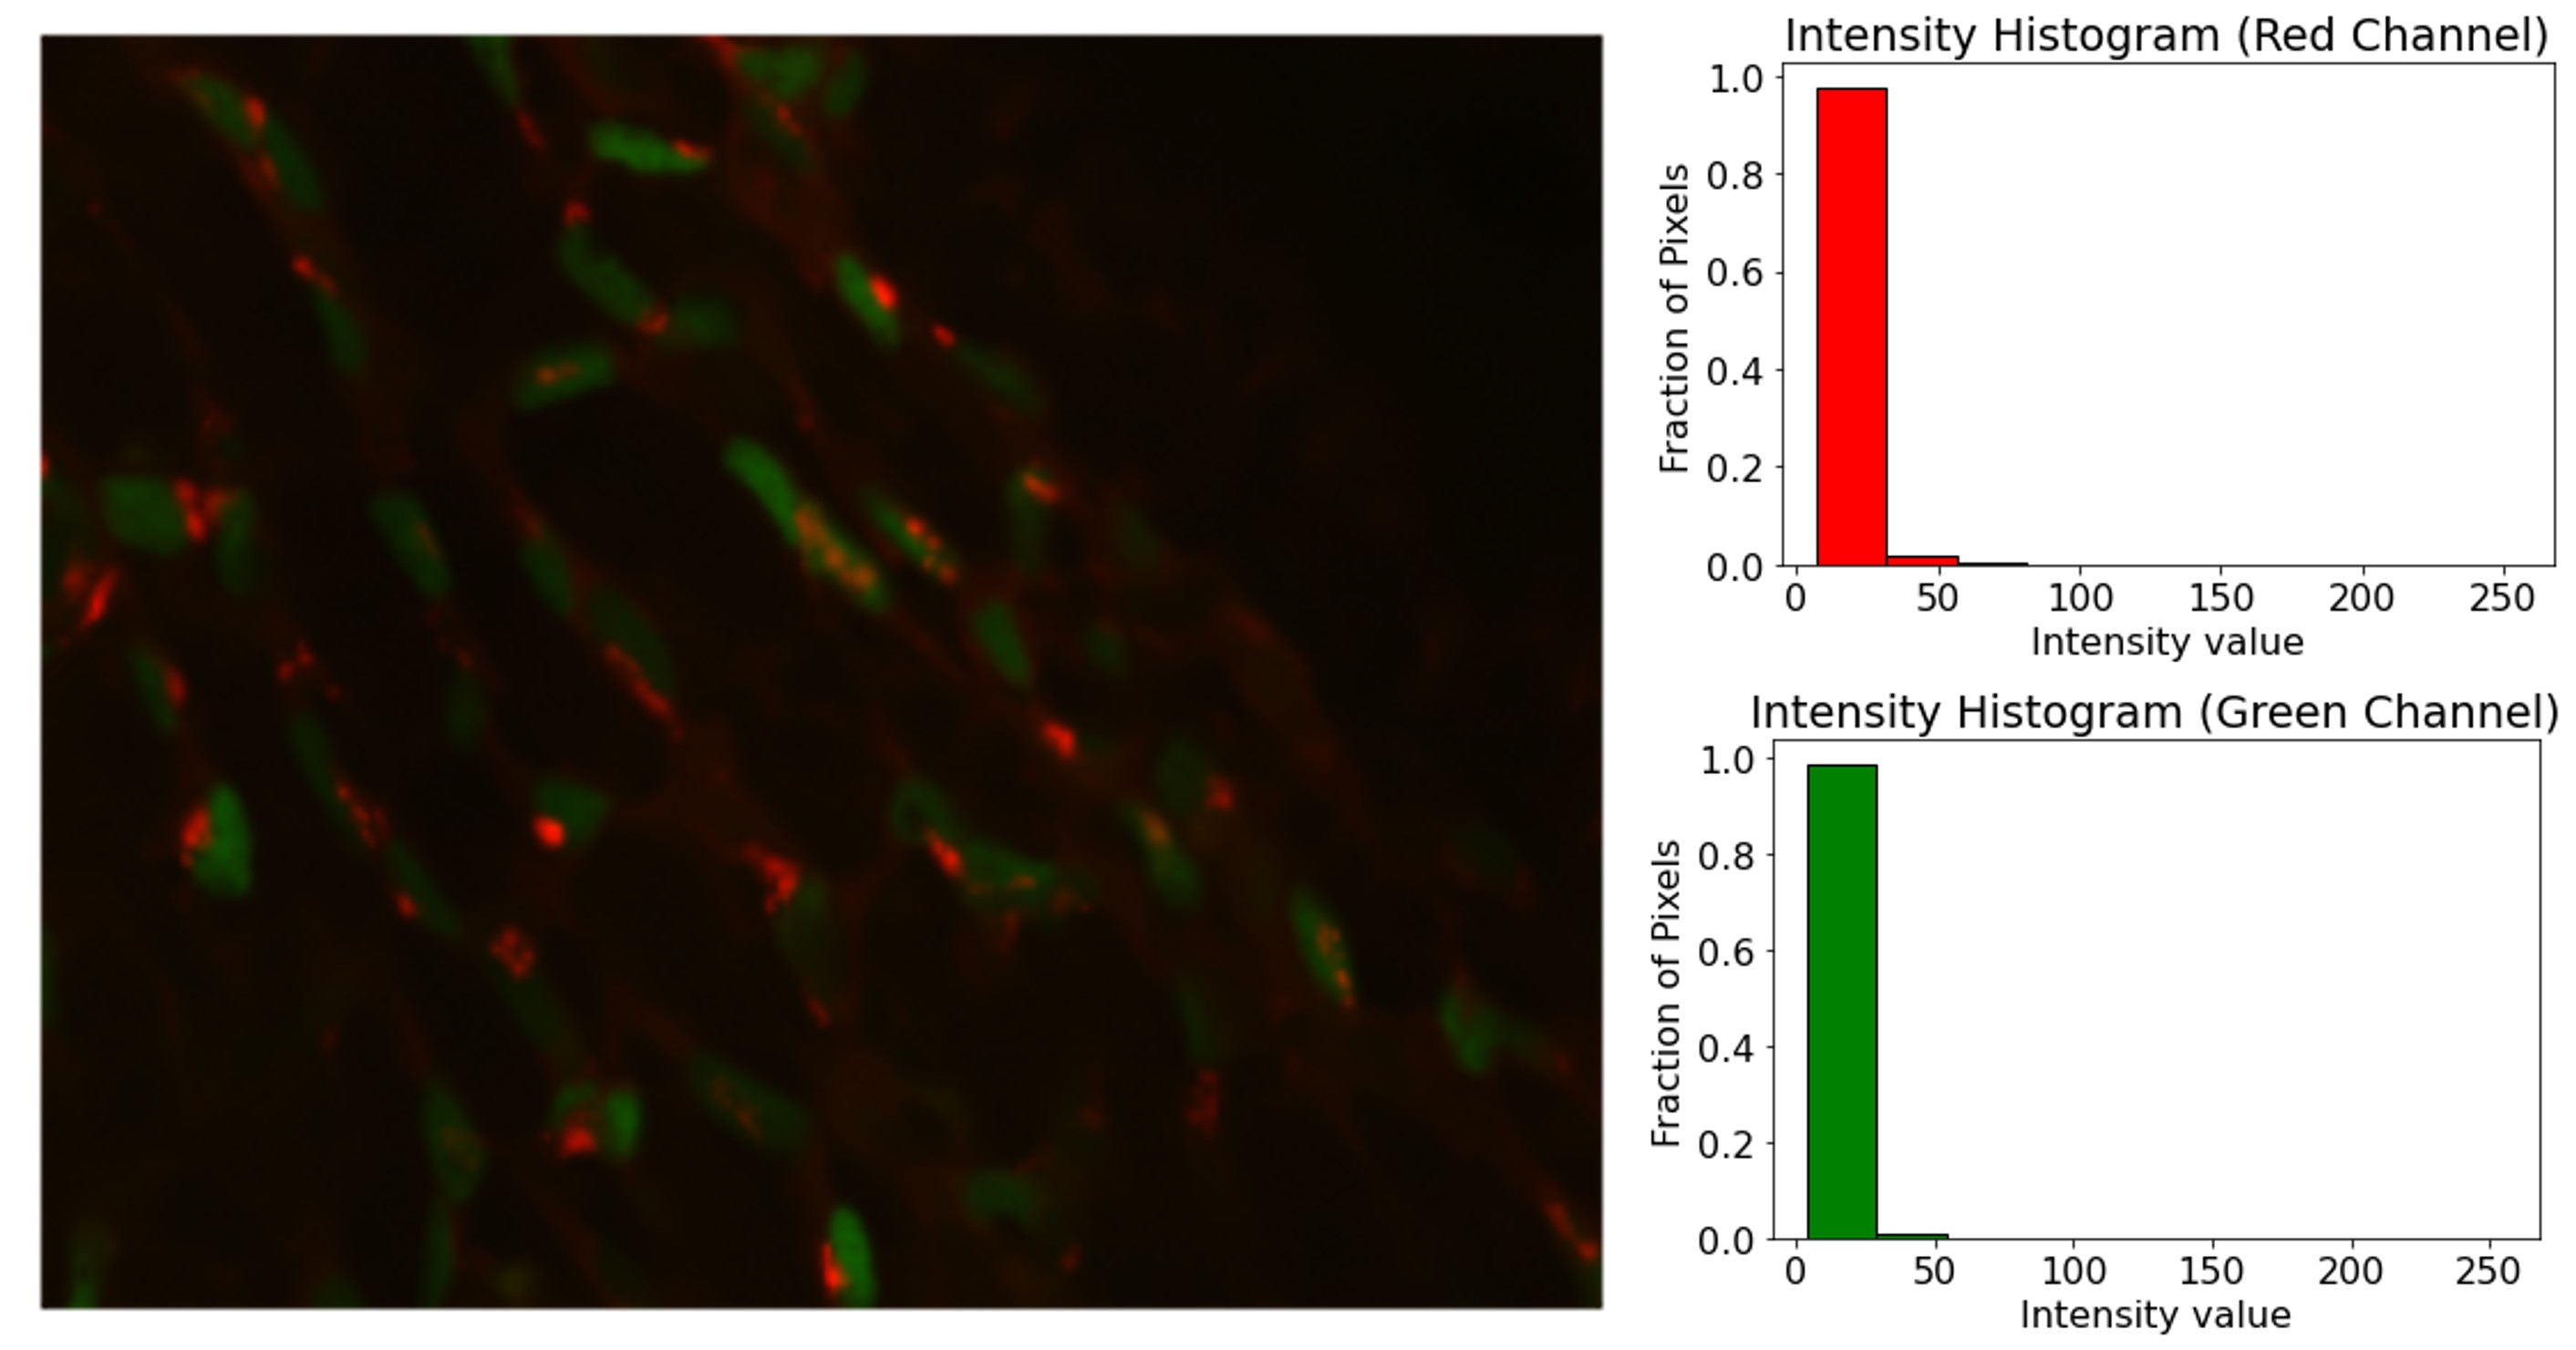
\includegraphics[width=0.75\textwidth]{Images/img.jpg}
  \caption[Slice of microscopic image from the dataset.]{Slice of microscopic image from the dataset.}
  \label{fig:micro}
\end{figure}

% https://www.notilyze.com/en/news/improving-object-detection-with-contrast-stretching-part-1-2/

Contrast stretching should theoretically improve the learning ability of models by highlighting the contours of objects and emphasizing the difference between object and background. This helps convolutional layers extract information and features from images \cite{contrast_strect}. Contrast stretching can be easily done for an image using a formula that scales up the differences in pixel values. This up scaling must be applied to all color channels, so for the microscopic images used in this work, it must be applied to the red and green channels (as mentioned earlier, these images have no blue channel).

The contrast stretching can be done by transforming pixel $x$ following formula:

\begin{equation}
    \label{eq:contrast}
    f(x) = \frac{x-a}{b-a} \times 255
\end{equation}


\noindent where $a$ is the lower limit to scale to, and $b$ is the upper limit. Instead of using the minimum and maximum values in the contrast stretch as the lower and upper bounds, the 5 and 98 percentile values are used, respectively. These values were chosen by visual inspection of the pre-processing results considering different percentile values. The values that best enhance the contrast of the Golgi and nuclei were selected.

The results of this process can be found in figure \ref{fig:micro_pre} and, together with the corresponding new intensity histograms for the red and green channels.

\begin{figure}[!htb]
  \centering
  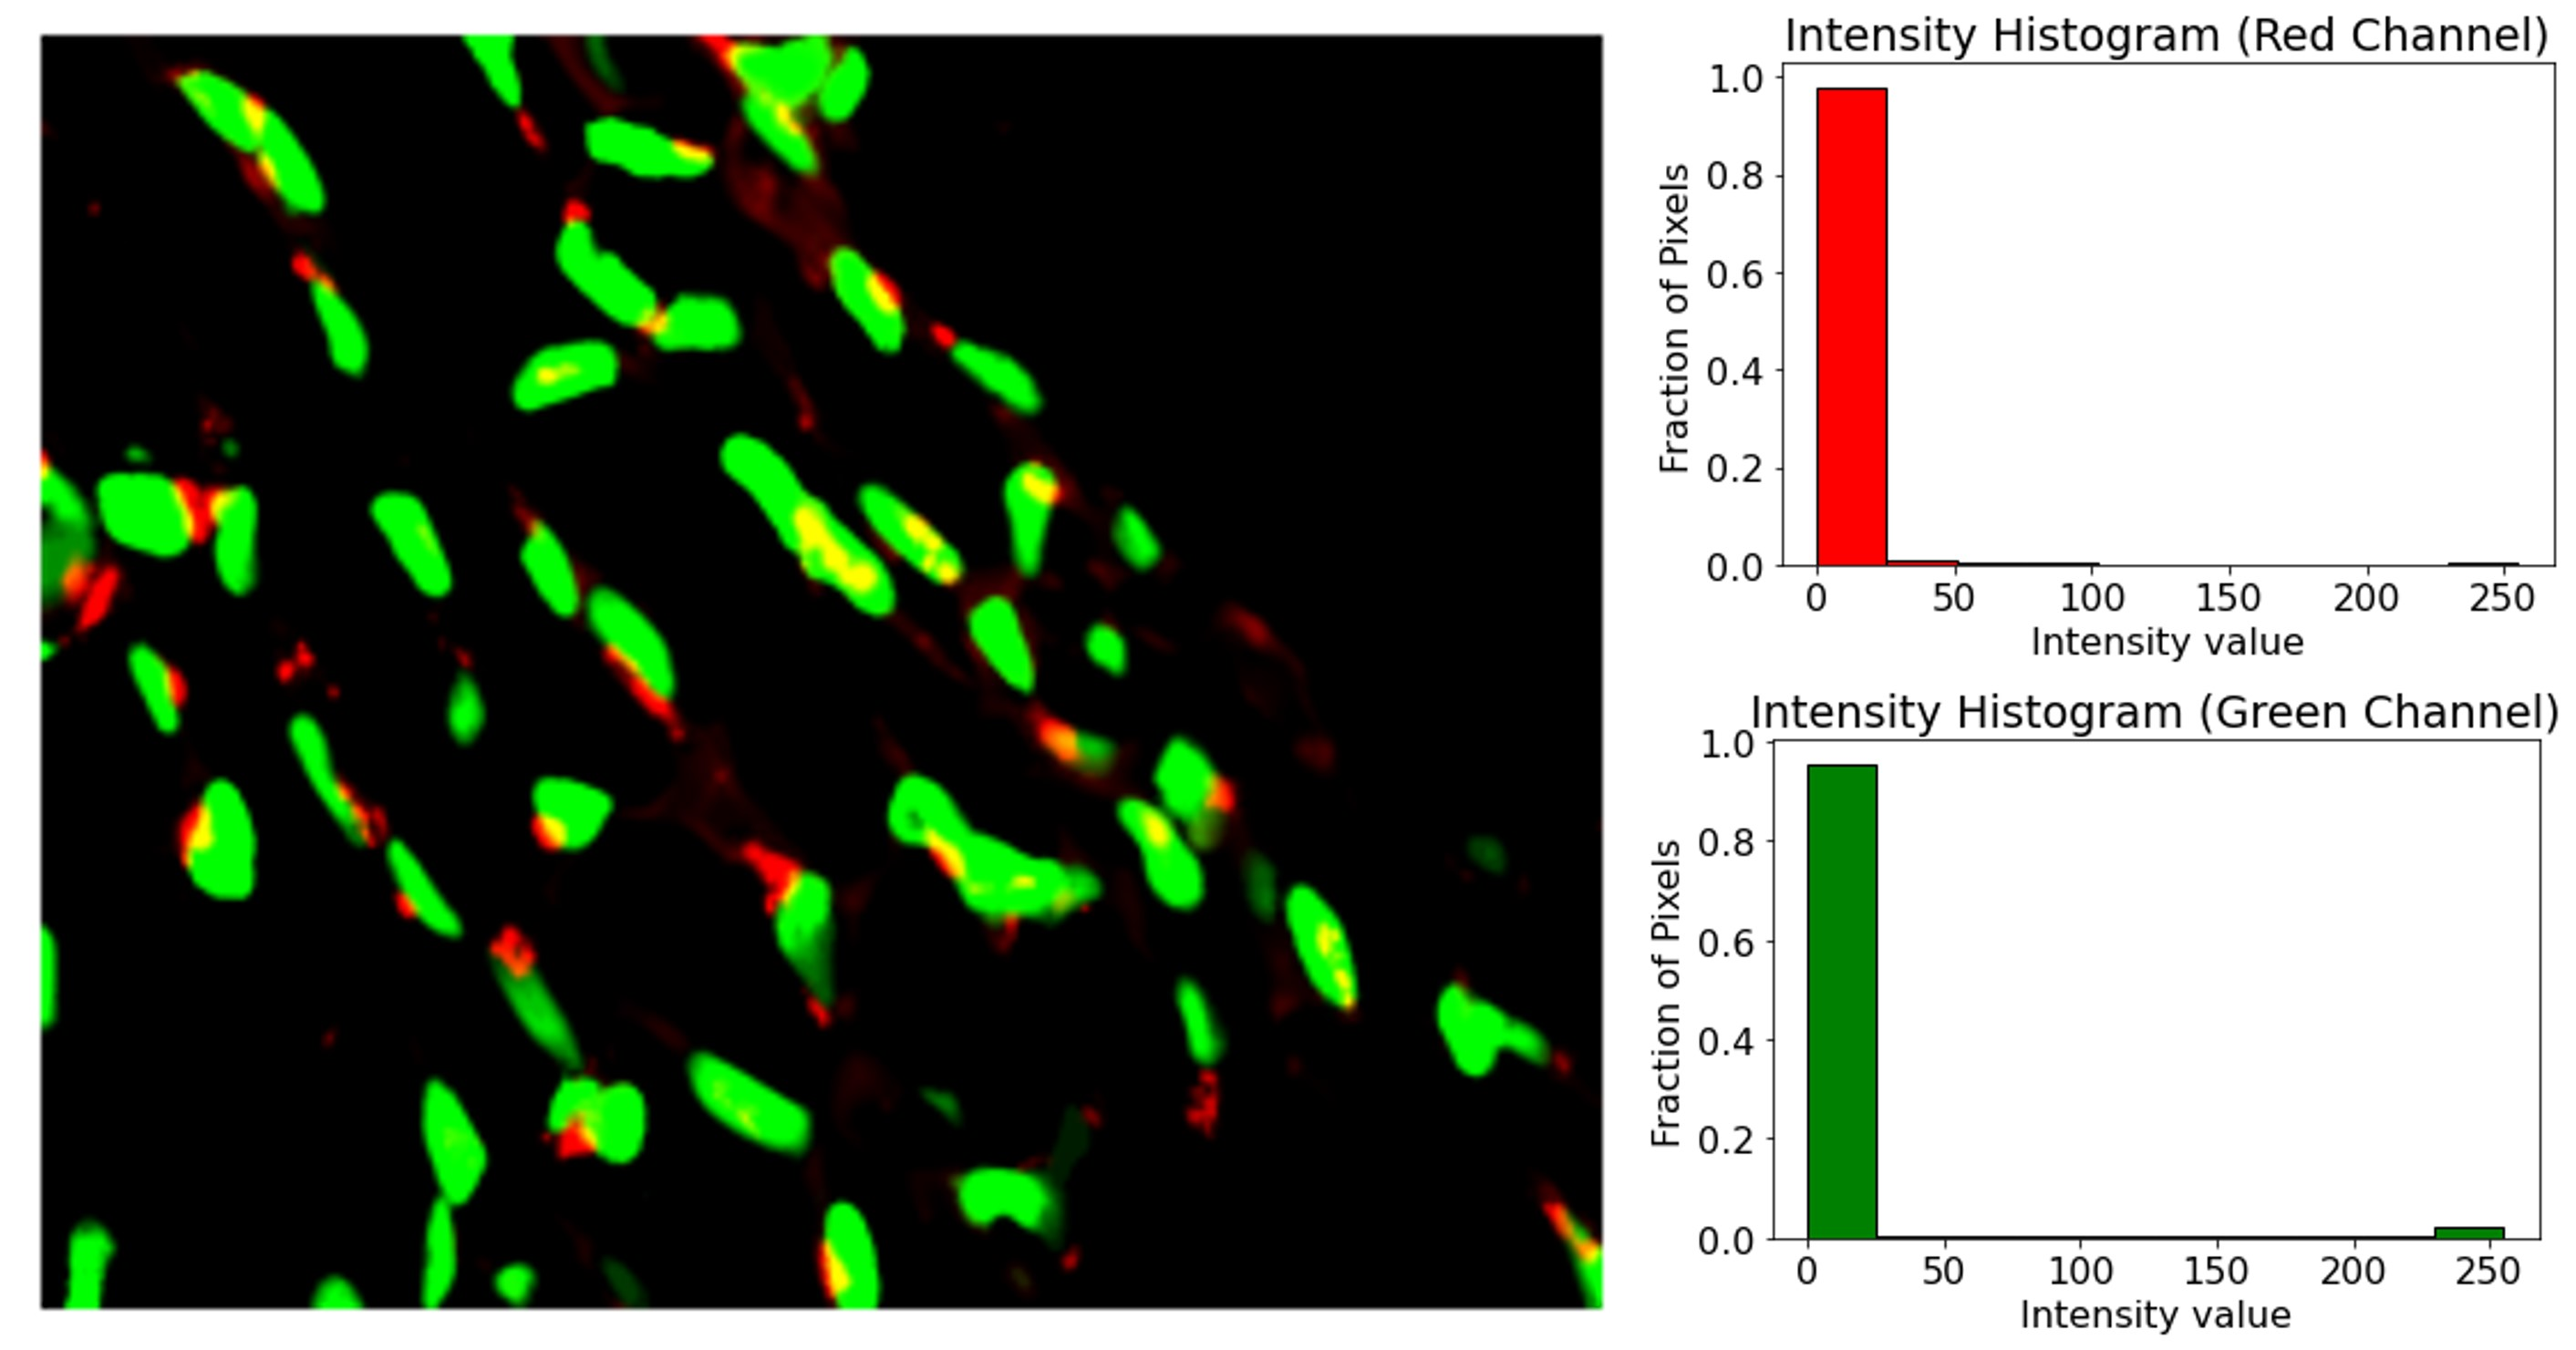
\includegraphics[width=0.75\textwidth]{Images/pre.jpg}
  \caption[Same image slice of figure \ref{fig:micro} after percentile contrast stretching.]{Same image slice of figure \ref{fig:micro} after percentile contrast stretching.}
  \label{fig:micro_pre}
\end{figure}


Another simple step of the data pre-processing method applied to the dataset of microscopic images was to normalize the input images with values in the range [0,255] to values in the interval [0,1] by dividing each image value by 255. This process is important because when the original images are used as input of the Deep Neural Networks, computing these high numerical values requires a lot of computational resources and time. When the data is normalized, the pixel values are smaller, so the computational resources and time required to converge the model are greatly reduced.

\section{Implementation Details, Results and Discussion}

In this section the experimental results regarding the segmentation of cell nuclei and Golgi in fluorescence microscopy images obtained with the proposed models are presented and discussed. In each subsection, a different model is described and each subsection is divided into two parts. In \textbf{2 Class}, the results obtained for the models predicting two output probability maps (for nuclei and Golgi) are presented, and in \textbf{3 Class}, the results obtained for the models predicting three output probability maps (nuclei, Golgi and nucleus-Golgi pairs) are presented.

All models are tested on two of the eight crops in the dataset described in section \ref{section:dataset}. Shown in figure \ref{fig:dataset} are: the original test crops in (a) and (e), designated $I^{orig}_1$ and $I^{orig}_2$, respectively; the crops obtained by applying the pre-processing method described in the previous section in (b) and (f), designated $I^{Pre}_1$ and $I^{Pre}_2$, respectively; the ground truth segmentation masks for the models with 2 output channels in (c) and (g), denoted $I^{gt}_{21}$ and $I^{gt}_{22}$, respectively; and the ground truth segmentation masks for the models with 3 output channels in (d) and (h), denoted $I^{gt}_{31}$ and $I^{gt}_{32}$, respectively.

\begin{figure}[!htb]
\centering
\subfigure[]{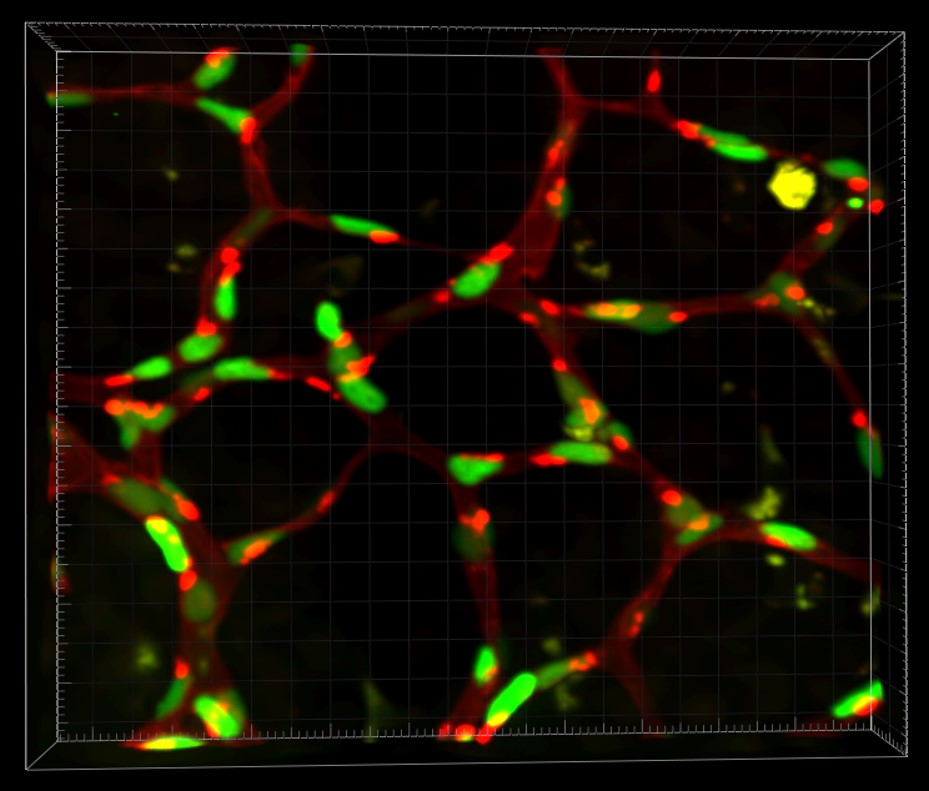
\includegraphics[width=3.5cm]{Images/crop5_img.jpg}}\hfil
\subfigure[]{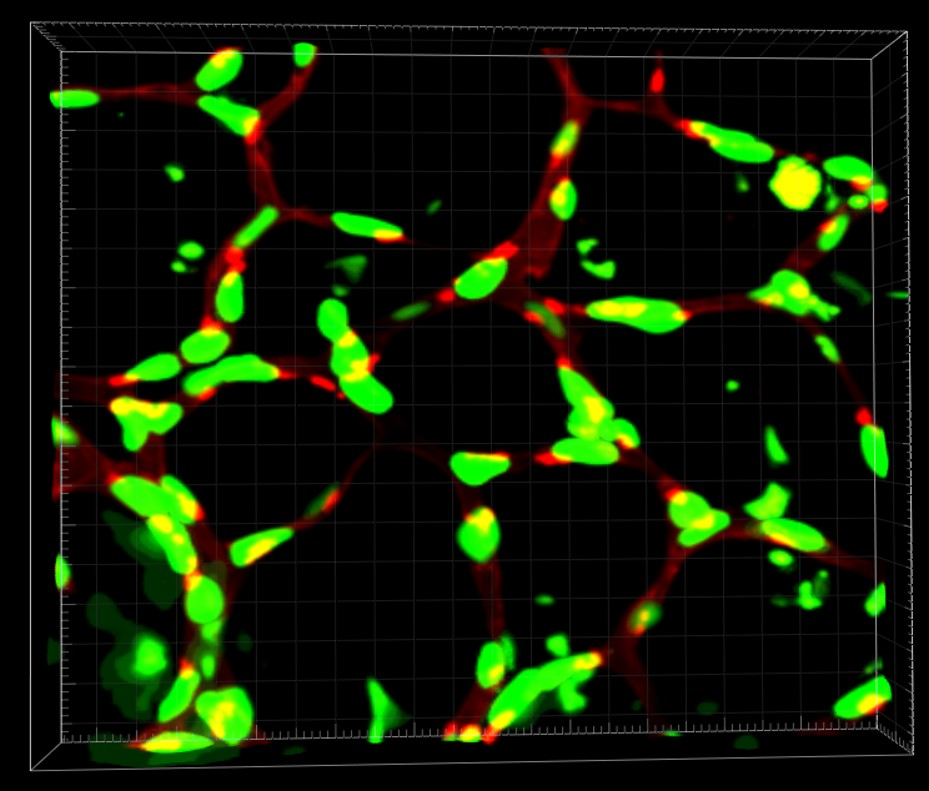
\includegraphics[width=3.5cm]{Images/pre_crop5_image.jpg}}\hfil 
\subfigure[]{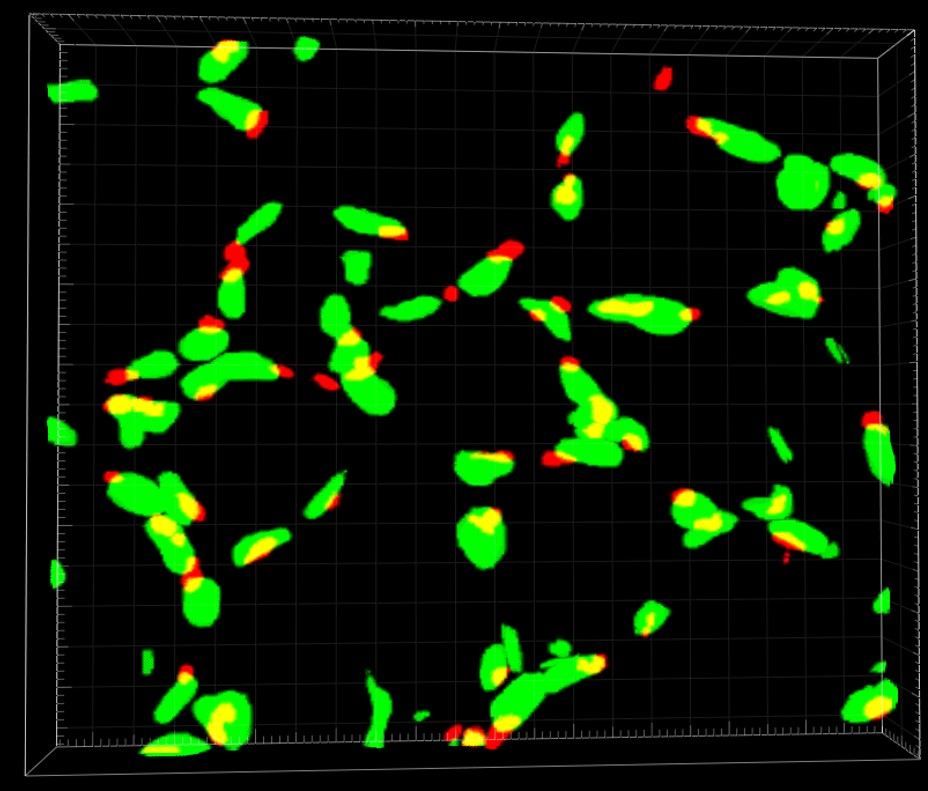
\includegraphics[width=3.5cm]{Images/2-mask-crop5.jpg}}\hfil
\subfigure[]{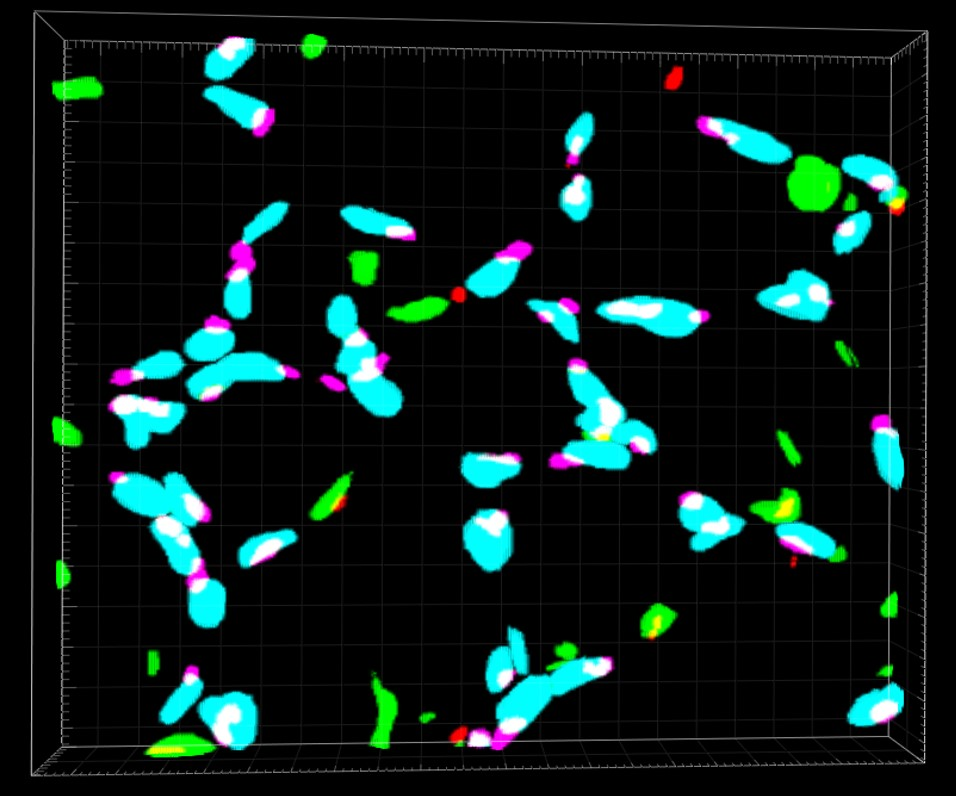
\includegraphics[width=3.5cm]{Images/3-mask-crop5-original.jpg}}

\subfigure[]{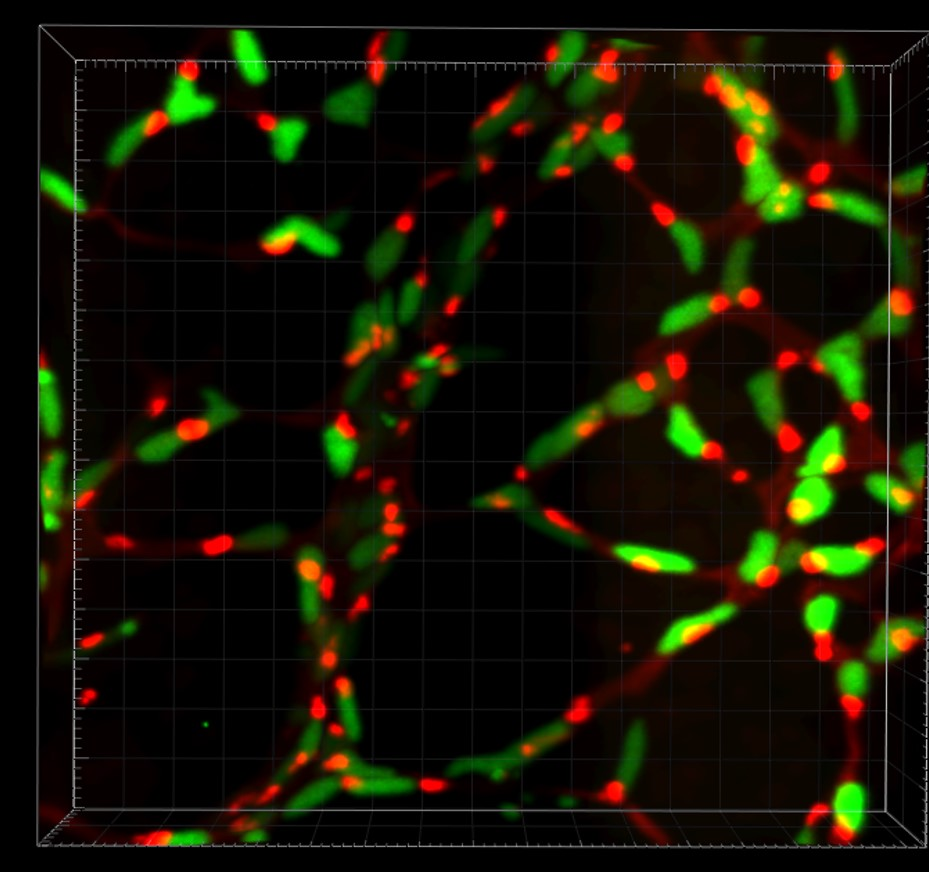
\includegraphics[width=3.5cm]{Images/crop7_img.jpg}}\hfil 
\subfigure[]{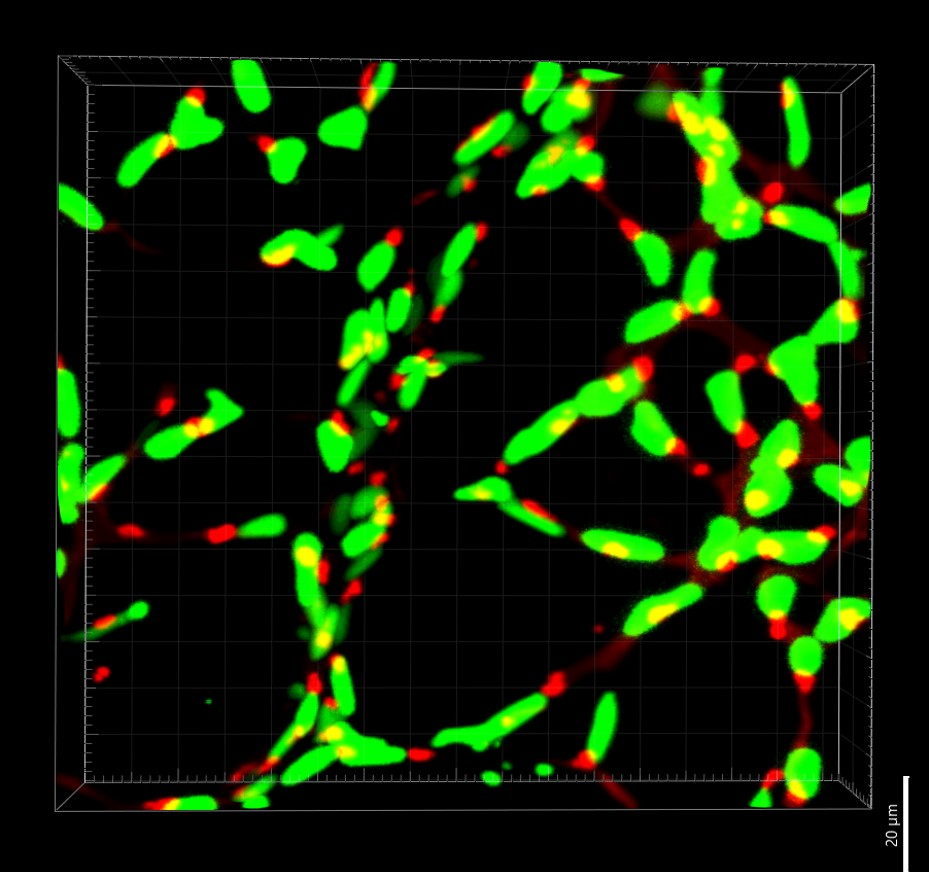
\includegraphics[width=3.5cm]{Images/pre_crop7_image.jpg}}\hfil
\subfigure[]{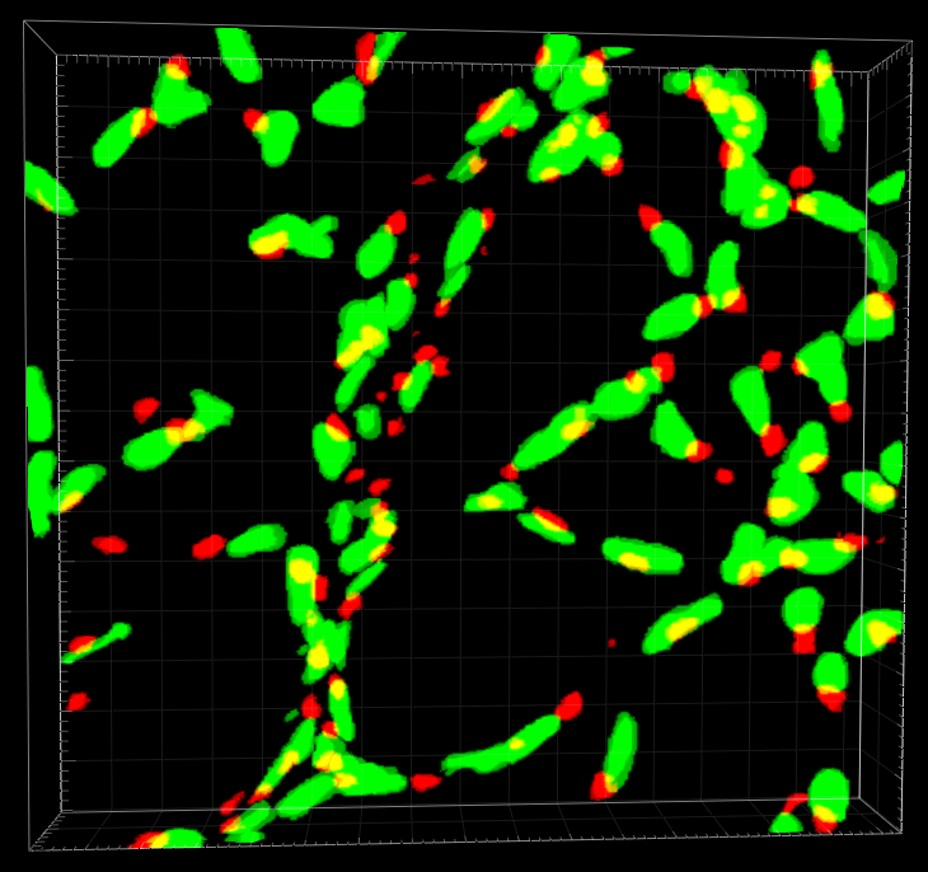
\includegraphics[width=3.5cm]{Images/2-mask-crop7.jpg}}\hfil
\subfigure[]{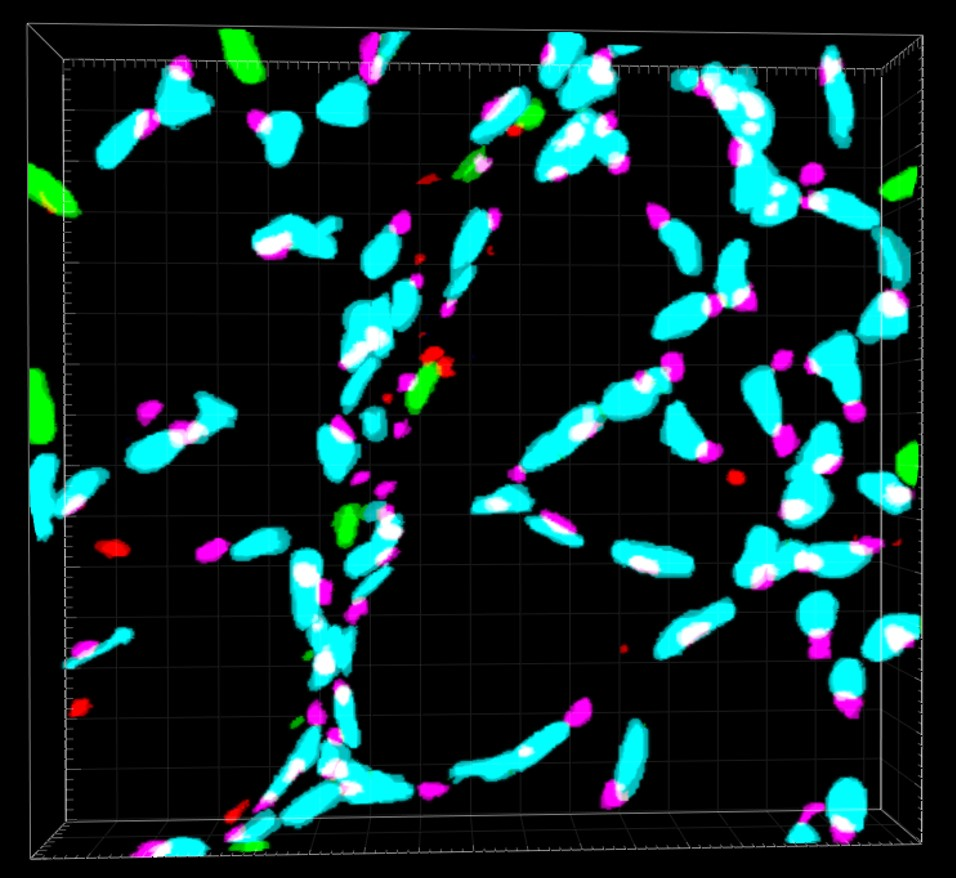
\includegraphics[width=3.5cm]{Images/3-mask-crop7-original.jpg}}
\caption{3D visualization of crops used for testing the models: (a) $I^{orig}_1$; (b) $I^{Pre}_1$; (c) $I^{gt}_{21}$; (d) $I^{gt}_{31}$; (e) $I^{orig}_2$; (f)  $I^{Pre}_2$; (g) $I^{gt}_{22}$; (h) $I^{gt}_{32}$.}

\label{fig:dataset}

\end{figure}

As mentioned in section \ref{section:dataset}, the crops for training the proposed models were divided into equal-sized patches. Therefore, the training dataset for all proposed models consists of 433 patches with a size of 64x64x64 from 6 different crops.

\subsection{3D U-Net}

In this subsection the results obtained by training and testing the 3D U-Net model are presented and discussed.

\subsubsection*{Implementation Details}

First, details on the choice of the model's hyperparameters are presented.

In all experiments, using the \ac{3D} U-Net model: Early stopping was applied to stop training when the validation loss did not improve for 10 epochs; the model was trained with the ADAM optimizer with a learning rate of 1e-3; using Xavier initialization for the model weights; a batch size of 4 and \ac{ReLU} as activation functions, except in the last layer, which has a sigmoid activation function so that the output is $n$-probability maps (where $n$ is the number of classes). A threshold of 0.5 is then applied to each probability map of the output of the U-Net to obtain the final segmentation mask.


\subsubsection*{2 Class}

The U-Net model was first trained with the original dataset (figure \ref{fig:micro}). The obtained segmentation masks for the experiment are shown in figures \ref{fig:results-unet} (b) and \ref{fig:results-unet} (e), and table \ref{tab:u-net-results} lists the values obtained for the metrics used to evaluate the model which were described in section \ref{section:metrics}.

From the results, it can be concluded that in the original dataset the precision of the nuclei and especially the Golgi is very low, which indicates over-segmentation and can be verified by looking at the obtained images. This also leads to a very low dice coefficient. Therefore, to improve these results, the pre-processing method described in the previous section \ref{section:pre} was applied to the microscopic images and the U-Net model was re-trained with patches extracted from the pre-processed images.

The segmentation masks obtained for the pre-processed microscopic images are shown in figures \ref{fig:results-unet} (c) and \ref{fig:results-unet} (f) and table \ref{tab:u-net-results} provides the values of the metrics used to evaluate the model. Compared to the previous results, the pre-processing method improved the results significantly, especially the precision and Dice Coefficient. However, it still tends to over-segment, especially the Golgi.

% Please add the following required packages to your document preamble:
% \usepackage{graphicx}
\begin{table}[!htb]
\centering
\caption{Average metric values after testing the 3D U-Net model on two microscopic images for a model trained with the original microscopic images (U-Net) and with the pre-processed microscopic images (U-Net + Pre)}
\label{tab:u-net-results}
\resizebox{\columnwidth}{!}{%
\renewcommand\arraystretch{1.4}
\begin{tabular}{c|c|c|c|c|c|c|}
\cline{2-7}
                                  & \multicolumn{1}{l|}{DC   Nuclei} & \multicolumn{1}{l|}{DC Golgi} & \multicolumn{1}{l|}{Precision Nuclei} & \multicolumn{1}{l|}{Precision Golgi} & \multicolumn{1}{l|}{Recall Nuclei} & \multicolumn{1}{l|}{Recall Golgi} \\ \hline
\multicolumn{1}{|c|}{U-Net}       & 0,4497                           & 0,3054                        & 0,2912                                & 0,1842                               & 0,9895                             & 0,9186                            \\ \hline
\multicolumn{1}{|l|}{U-Net + Pre} & 0,7775                           & 0,6938                        & 0,7067                                & 0,6500                               & 0,8692                             & 0,7683                            \\ \hline
\end{tabular}%
}
\end{table}

\begin{figure}[!htb]
  
\centering
\subfigure[]{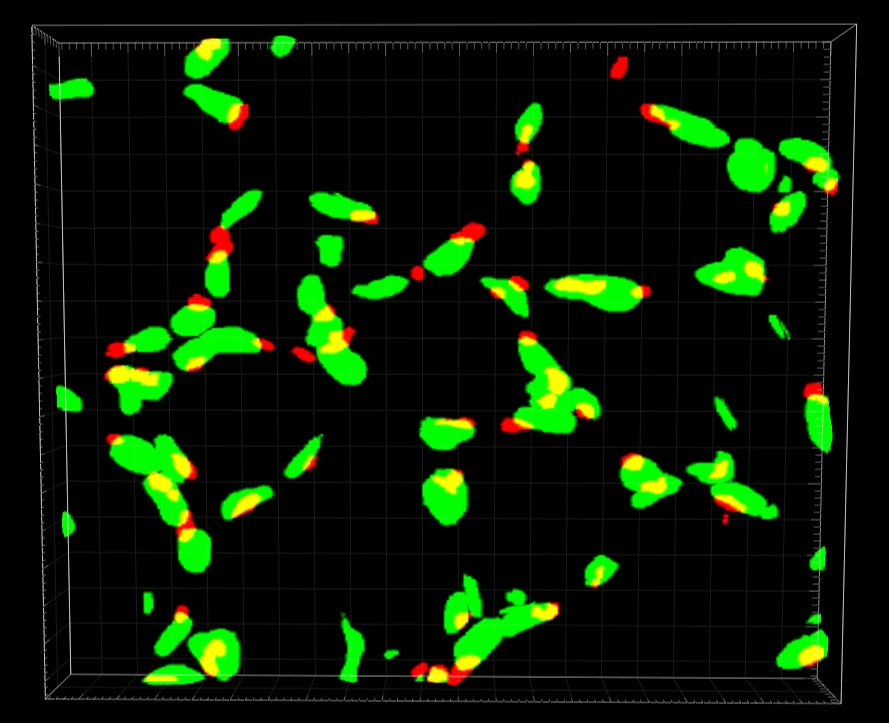
\includegraphics[width=4.5cm]{Images/mask-crop5.jpg}}\hfil
\subfigure[]{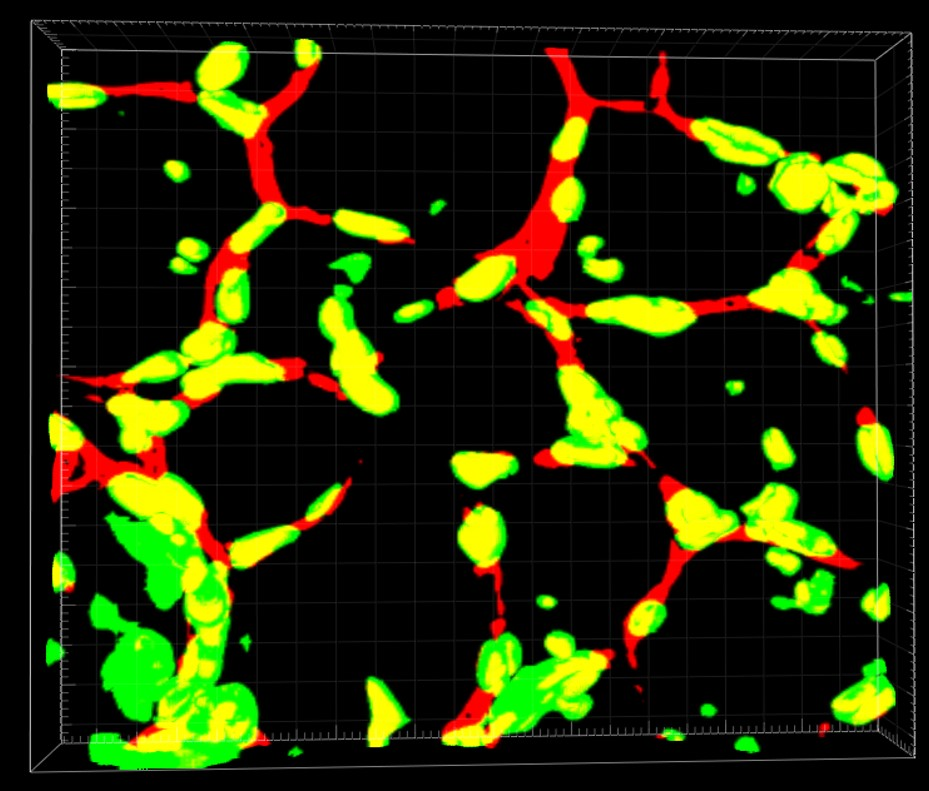
\includegraphics[width=4.5cm]{Images/u-net-crop5-not-pre.jpg}}\hfil 
\subfigure[]{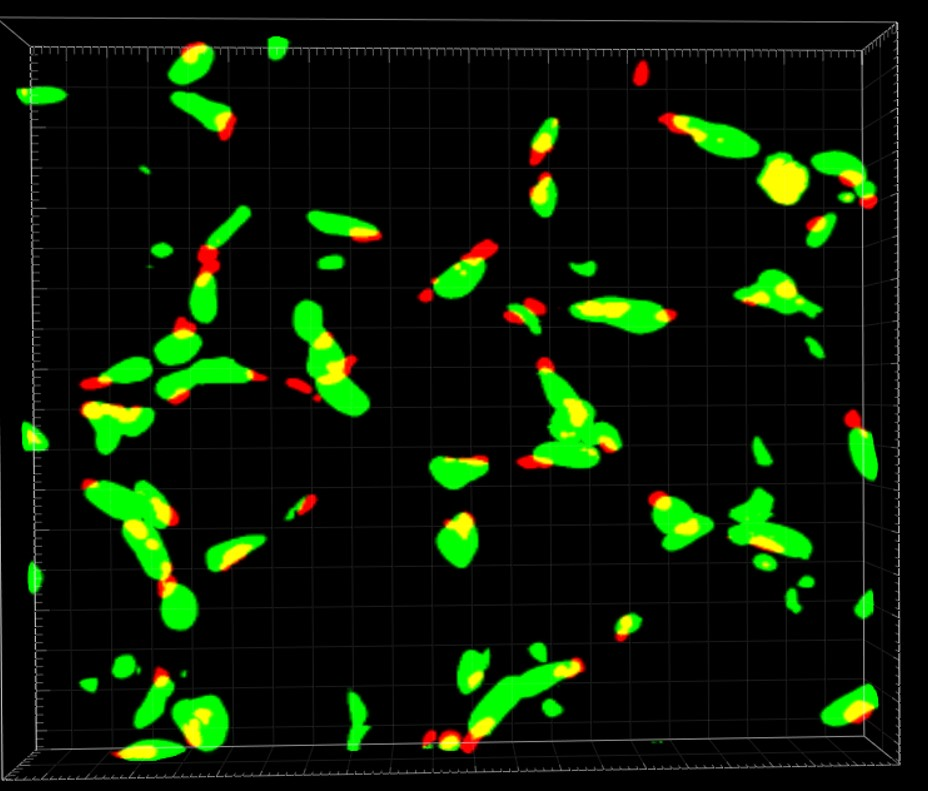
\includegraphics[width=4.5cm]{Images/u-net-aft-pre-crop5.jpg}} 

\subfigure[]{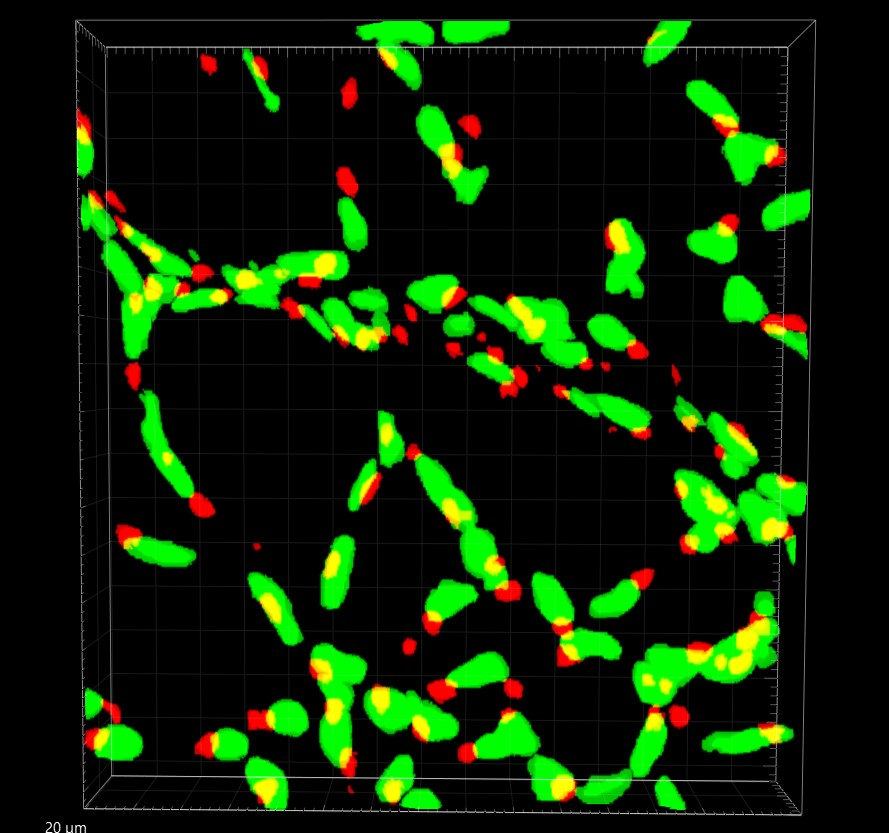
\includegraphics[width=4.5cm]{Images/mask-crop7.jpg}}\hfil 
\subfigure[]{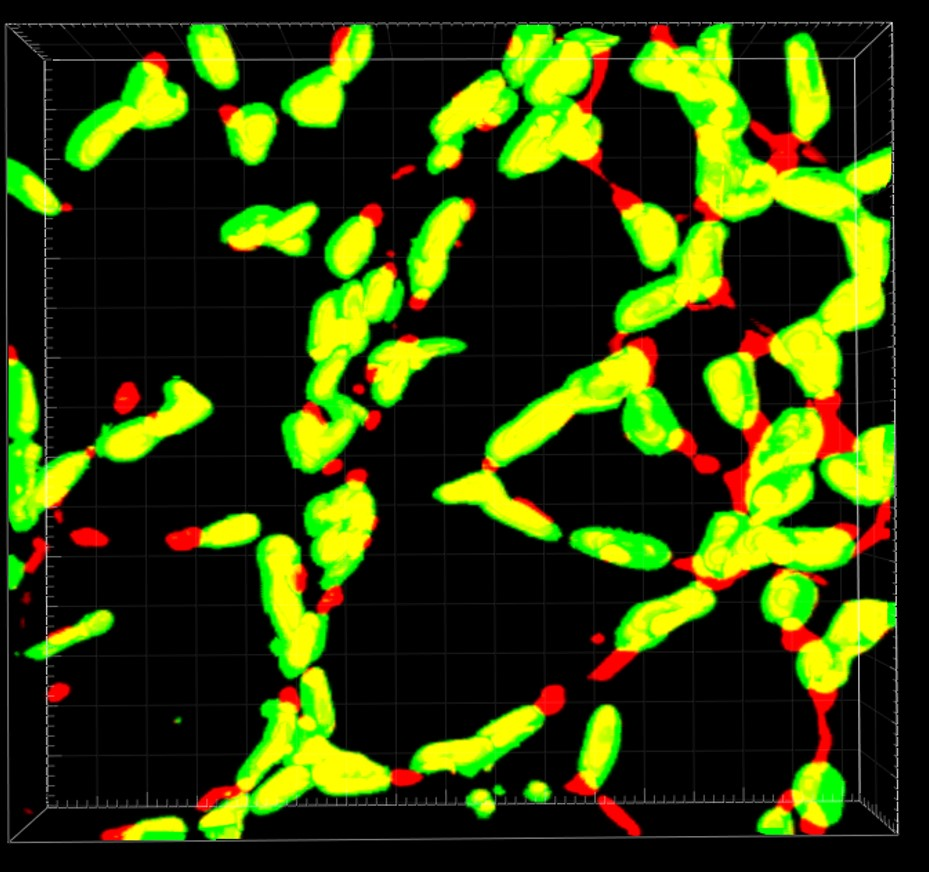
\includegraphics[width=4.5cm]{Images/u-net-crop7-not-pre.jpg}}\hfil
\subfigure[]{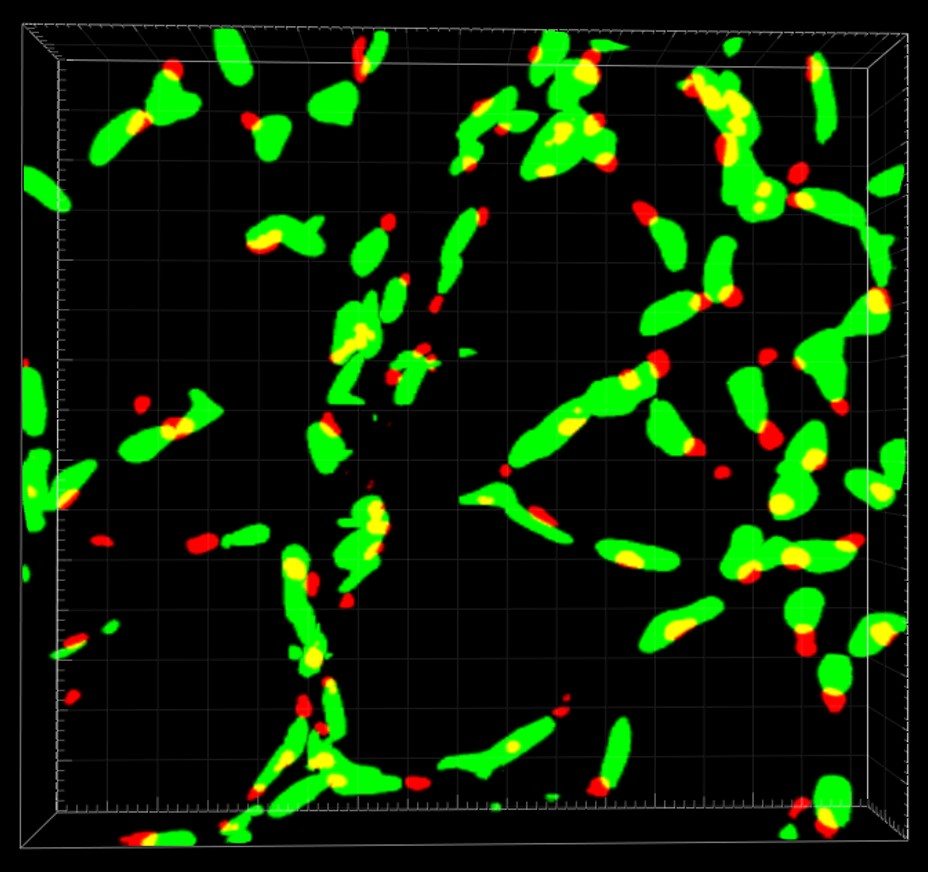
\includegraphics[width=4.5cm]{Images/u-net-aft-pre-crop7.jpg}}
\caption{3D visualization of segmentation masks: (a) 3D ground truth $I^{gt}_{21}$; (b) 3D U-Net model tested on $I^{orig}_1$; (c) 3D U-Net model tested on $I^{Pre}_1$; (d) 3D ground truth $I^{gt}_{22}$; (e) 3D U-Net model tested on $I^{orig}_2$; (f) 3D U-Net model tested on $I^{Pre}_2$.}

\label{fig:results-unet}

\end{figure}

There are two things that have been identified in the dataset that may lead to decreased precision of the model. The microscopic images have digital noise, which causes the model to classify this noise as Golgi/Nuclei. This has been verified specifically for the Golgi, and an example of this noise can be seen in figures \ref{fig:errors-unet} (d) to (f) highlighted by the blue circles. Another reason that leads to lower precision is that the manual segmentation masks contain annotation/segmentation errors. In figures \ref{fig:errors-unet} (a) to (c), we see that a Golgi is not identified in the segmentation mask  of our dataset, even though it is present in the microscopic image along with the nucleus and is identified correctly by the U-Net model.

The low recall can be explained by the fact that the microscopic images have low contrast in certain areas, even after applying the pre-processing method to the images. This causes the model to fail to recognise some Golgi/nuclei, which lowers the recall. This case is illustrated in figure \ref{fig:errors-unet} (d) to (e) by the orange circle.

\begin{figure}[!htb]

\centering
\subfigure[]{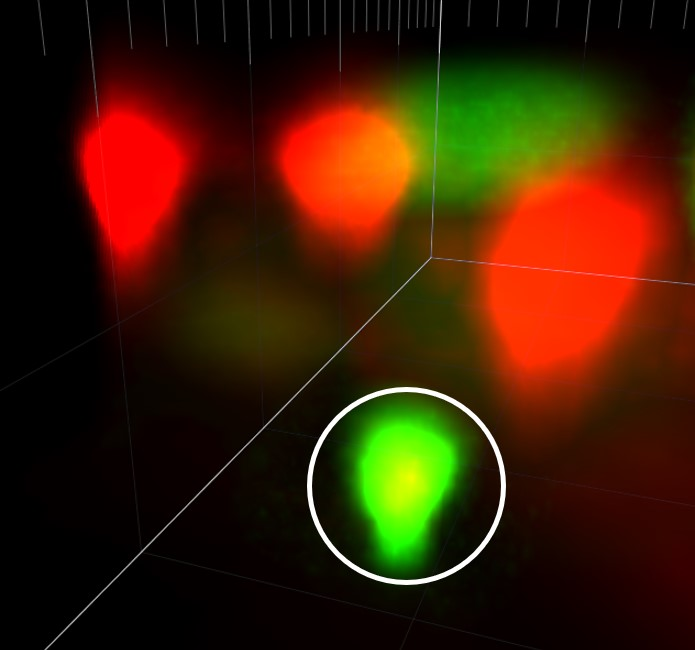
\includegraphics[width=4cm]{Images/image_noise.jpg}}\hfil
\subfigure[]{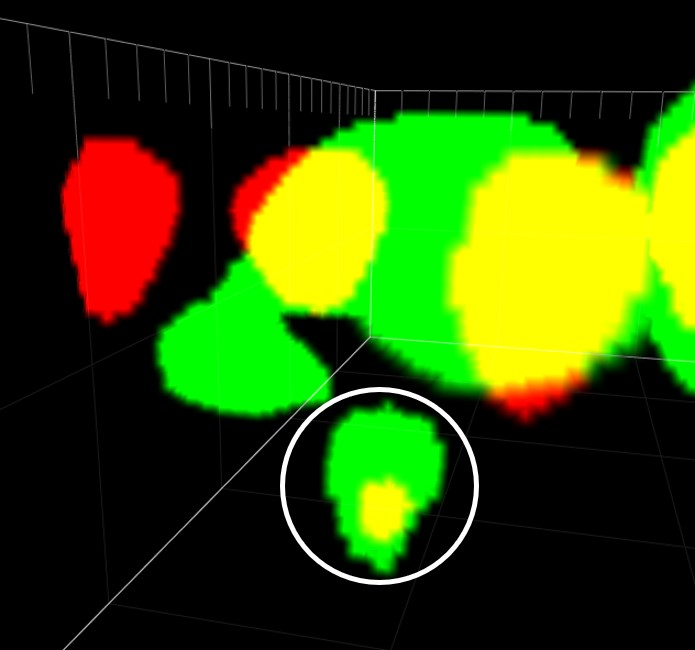
\includegraphics[width=4cm]{Images/my_mask_noise.jpg}}\hfil 
\subfigure[]{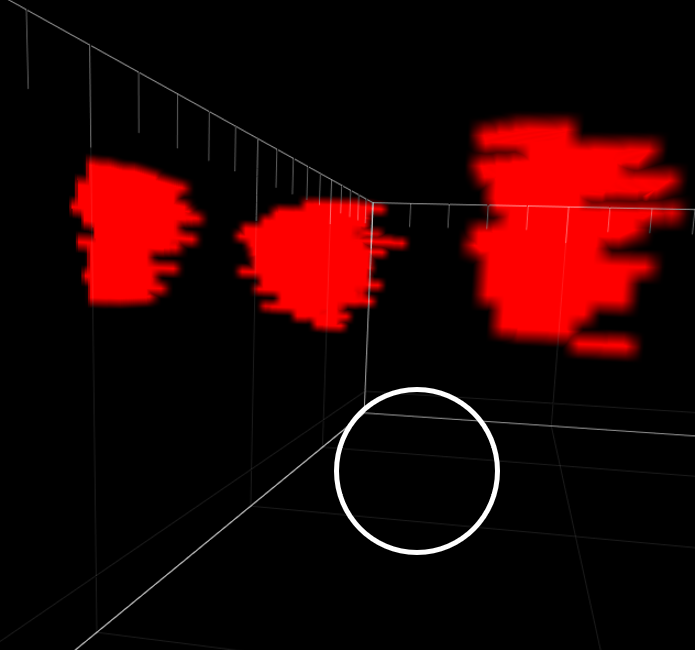
\includegraphics[width=4cm]{Images/real_mask_noise.jpg}} 

\subfigure[]{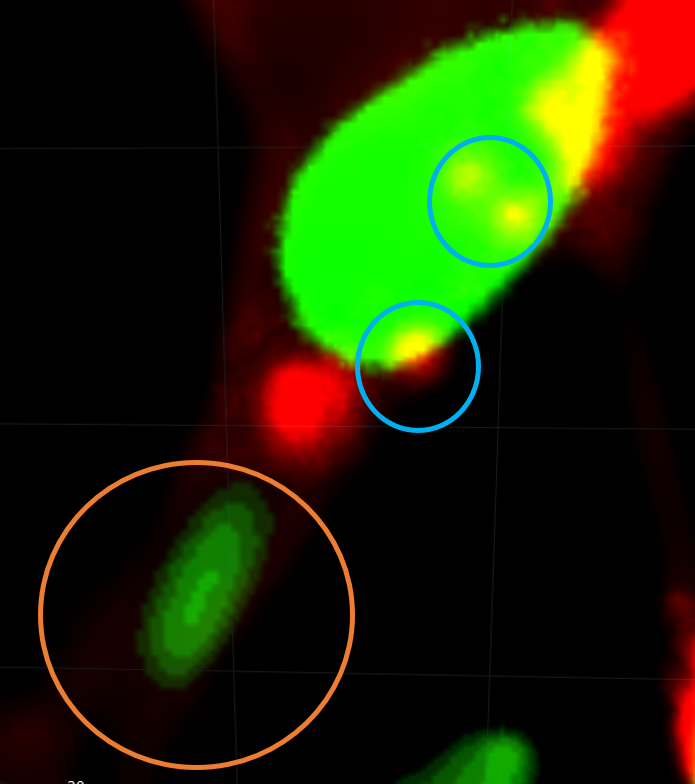
\includegraphics[width=4cm]{Images/noise_recall_image.jpg}}\hfil   
\subfigure[]{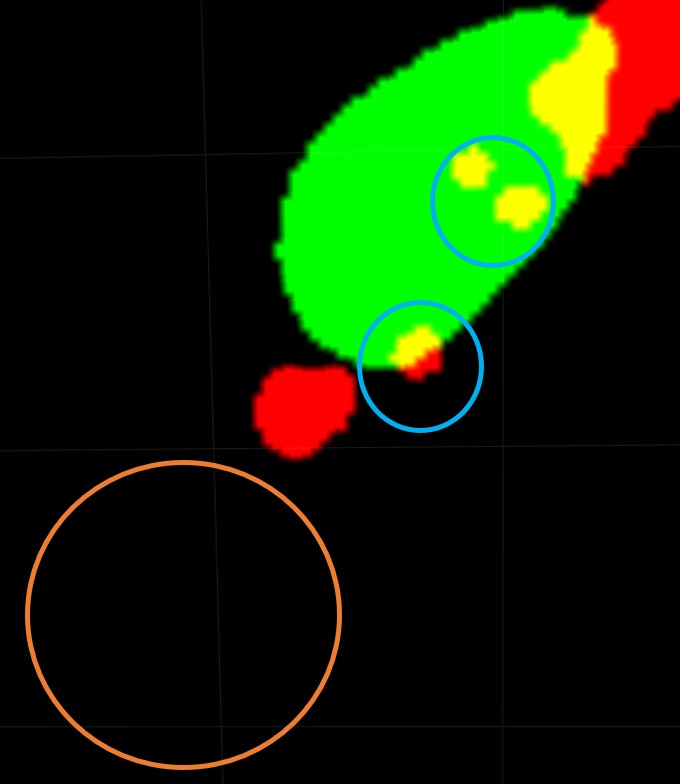
\includegraphics[width=4cm]{Images/noise_recall_my_mask.jpg}}\hfil
\subfigure[]{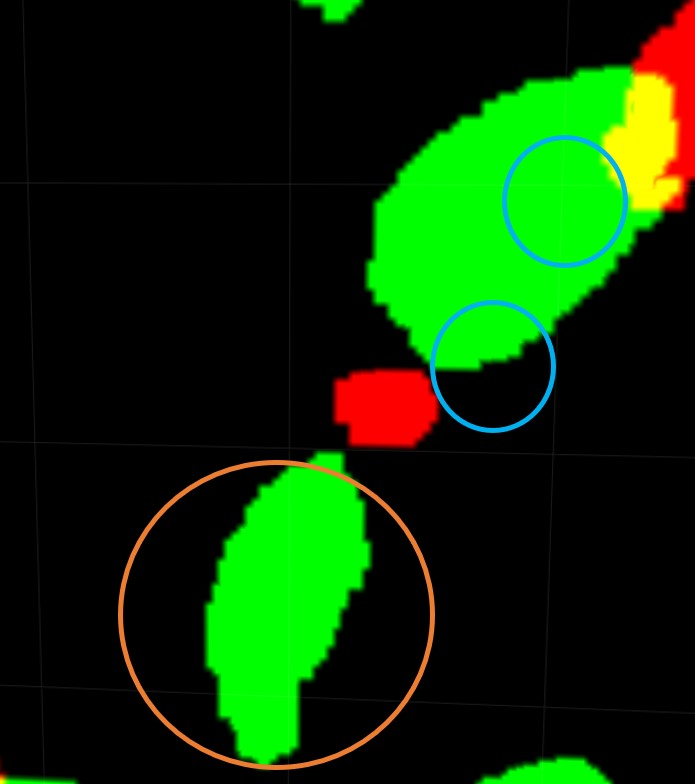
\includegraphics[width=4cm]{Images/noise_recall_real_mask.jpg}}
\caption{Example of ground truth mask imperfection highlighted by white circle; Example of digital noise highlighted by blue circles; and example of nondetection by 3D U-Net model highlighted by orange circle; (a) and (d) 3D microscopic section; (b) and (e) 3D U-Net segmentation mask; (c) and (f) 3D ground truth segmentation mask.}
\label{fig:errors-unet}



\end{figure}

To improve the results, different loss functions were tried to better segment the nuclei and Golgi, which would account for the imbalance between the background and the nuclei/Golgi, for example Focal Loss \cite{focal_loss}, but this did not lead to better results, instead caused the model to detect more noise. Another attempt was made by increasing the size of the data by applying transformations such as rotations and flips (reflections) to patches of the pre-processed dataset, but again this also did not produce better results but resulted in the model detecting more noise.

\subsubsection*{3 Class}

In this approach, the number of output probability maps of the 3D U-Net is three, so we can classify the nuclei, Golgi and nucleus-Golgi pairs of the input images. All other parameters described in the implementation details are kept. The model is trained with the pre-processed dataset and respective ground truth masks.

After training, the performance of the model is tested with the two microscopic image volumes $I^{Pre}_1$ and $I^{Pre}_2$. Figure \ref{fig:results-unet-3channel} is a 3D visualization of the segmentation results for these volumes and table \ref{tab:results-3class-u-net} shows the average quantitative results.

\begin{figure}[!htb]
\centering
\subfigure[]{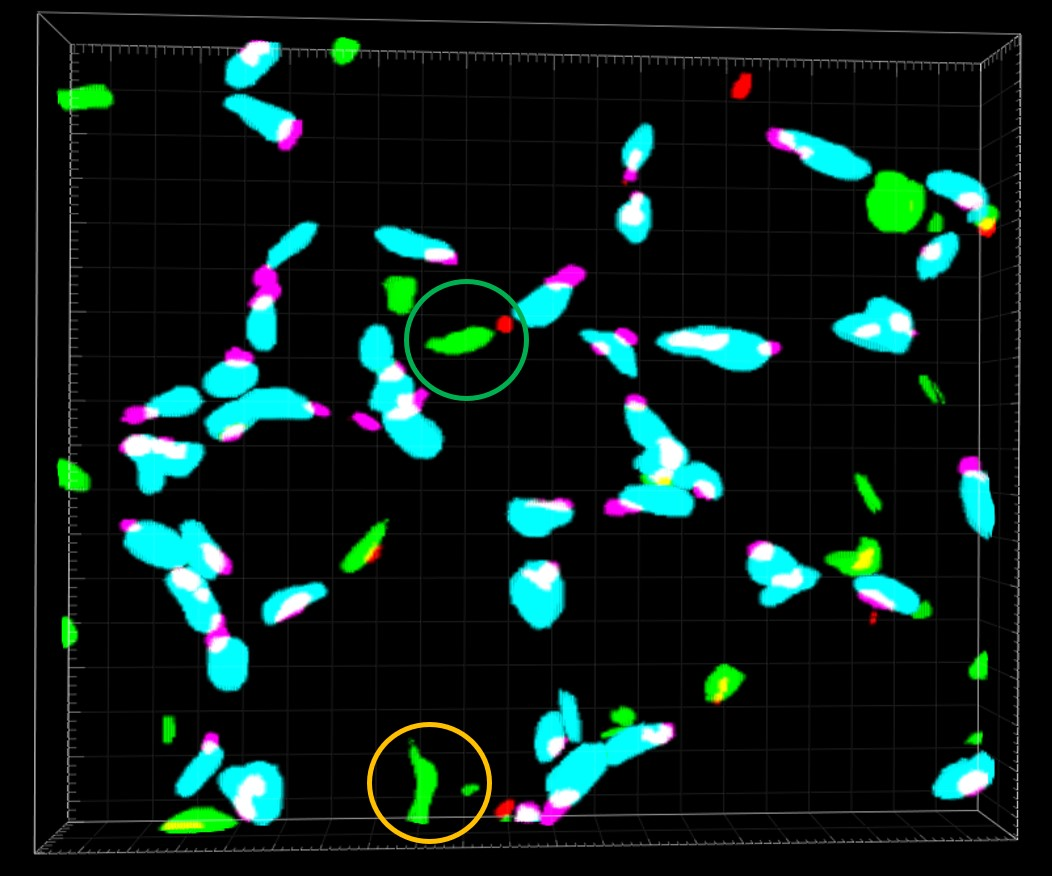
\includegraphics[width=5cm]{Images/3-mask-crop5.jpg}}\hfil
\subfigure[]{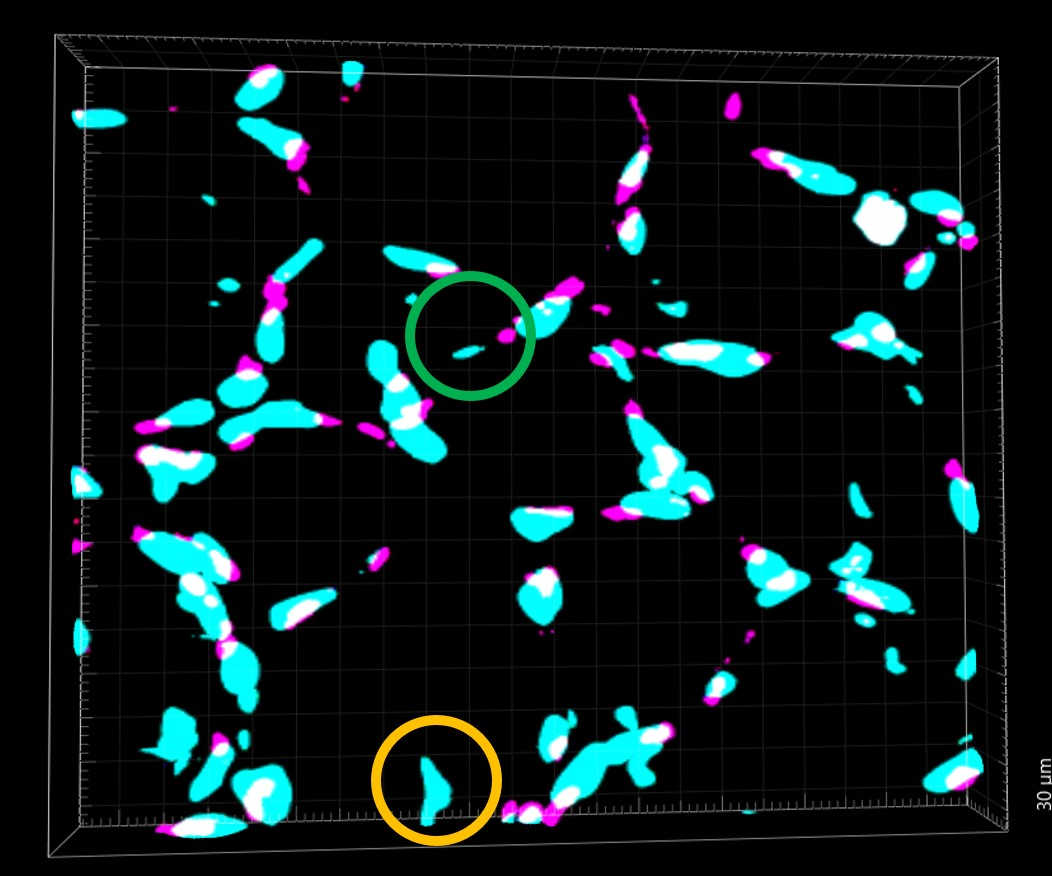
\includegraphics[width=5cm]{Images/u-net-3class-crop5.jpg}}

\subfigure[]{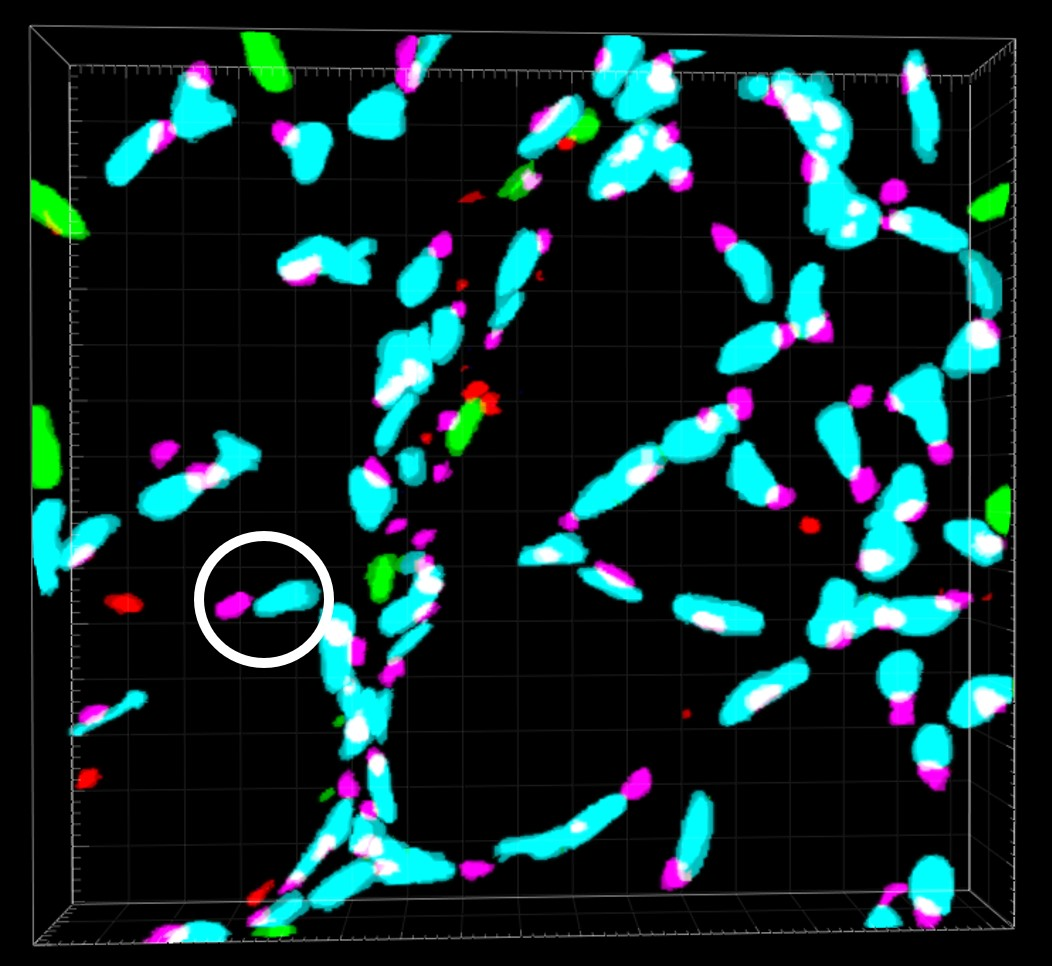
\includegraphics[width=5cm]{Images/3-mask-crop7.jpg}}\hfil 
\subfigure[]{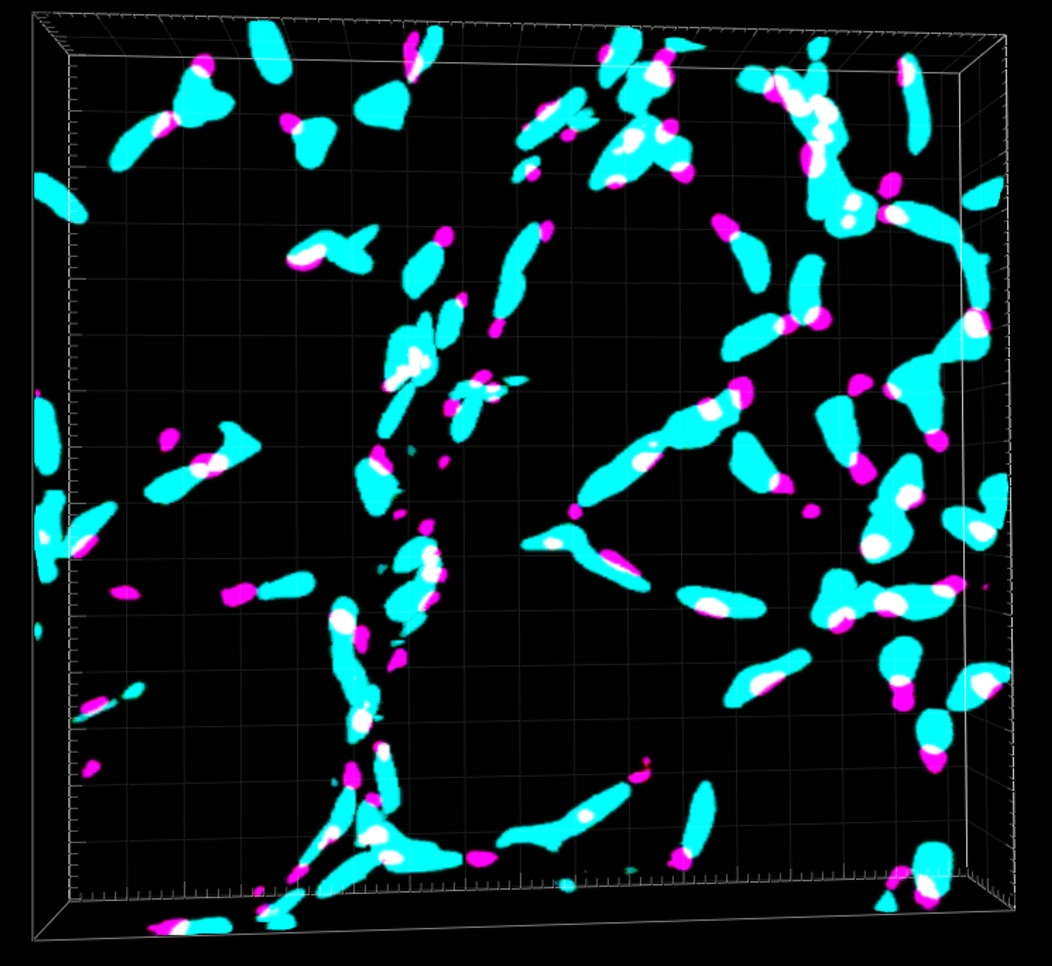
\includegraphics[width=5cm]{Images/u-net-3class-crop7.jpg}}

\caption{3D visualization of segmentation masks: (a) 3D ground truth $I^{gt}_{31}$; (b) 3 class 3D U-Net model tested on $I^{Pre}_1$; (c) 3D ground truth $I^{gt}_{32}$; (d) 3 class 3D U-Net model tested on $I^{Pre}_2$.}

\label{fig:results-unet-3channel}

\end{figure}

% Please add the following required packages to your document preamble:
% \usepackage{graphicx}
\begin{table}[!htb]
\centering
\caption{Average metric values after testing the 3 class 3D U-Net model on two pre-processed microscopic images}
\label{tab:results-3class-u-net}
\resizebox{\columnwidth}{!}{%
\renewcommand\arraystretch{1.4}
\begin{tabular}{|c|c|c|c|c|c|c|c|c|}
\hline
DC Nuclei & DC Golgi & DC Pair & Precision Nuclei & Precision Golgi & Precision Pair & Recall Nuclei & Recall Golgi & Recall Pair \\ \hline
0,7916    & 0,6752   & 0,7601  & 0,7589           & 0,5935          & 0,6941         & 0,8278        & 0,8206       & 0,8403      \\ \hline
\end{tabular}%
}
\end{table}

From Table \ref{tab:results-3class-u-net} we can see that, as expected, the Dice Coefficient, precision, and recall for the nuclei and Golgi classes are comparable to the values obtained previously. Looking at the results for the nucleus-Golgi pairs class, we can see from the segmentation masks in figure \ref{fig:results-unet-3channel} that the model is generally able to correctly identify this class, as reflected by a recall of 0.8403. However, the yellow circles in figure \ref{fig:results-unet-3channel} mark cases where the model is apparently unable to distinguish that an isolated nucleus or Golgi are not part of a pair and therefore should not be identified in the segmentation mask for the nucleus-Golgi pairs. Therefore, it also detects a lot of digital noise, which is reflected in the lower precision of 0.6941. The reason the model cannot learn these cases could be that these cases of isolated nuclei and Golgi are relatively rare and do not occur often enough in the dataset for the model to distinguish them.

As mentioned above, the ground truth mask for the Golgi and the nuclei has some imperfections. The main one is the fact that in the cases where the nuclei and the Golgi pairs do not overlap, no connection is made between them, which makes it difficult for the model to distinguish, for example, an isolated Golgi from a paired one. An example of this case is highlighted by the white circle in figure \ref{fig:results-unet-3channel}. Additionally, some of the nucleus-Golgi pairs are not annotated in the ground truth masks, but are correctly identified by the model, which also affects the precision results for the nucleus-Golgi pairs class. An example of this case is highlighted by a green circle in figure \ref{fig:results-unet-3channel}.

\subsection{Vox2Vox}

In this subsection the results obtained by training and testing the Vox2Vox model are presented and discussed.

\subsubsection*{Implementation Details}

As mentioned earlier, the Vox2Vox model consists of two networks, a generator and a discriminator. The discriminator is used only to improve the training, the generator is the segmentation network we want to obtain. In these two networks, the following specifications were set for training: He normal initialization for the model weights; the Adam Optimizer with a learning rate of 2e-5; batch size of 4 and early stopping to stop training when the validation loss did not improve for 20 epochs, saving the weights of the best model based on the lowest validation loss.

Specifically for the Vox2Vox generator, the sigmoid activation function was used in the last layer so that the output has $n$-probability maps (where $n$ is the number of classes). A threshold of 0.5 is then applied to each probability map of the output of Vox2Vox to obtain the final segmentation mask volume. The hyper-parameter $\alpha$ from the generator loss defined previously in equation \ref{eq:vox2vox-generator-loss} is set to $\alpha = 5$ as proposed in \cite{vox2vox}.

In a first phase, the model was trained with a loss function for the generator that gave the same weight to the nuclei and Golgi. However, with this loss function, the model had great difficulty detecting the Golgi on the images. This is likely due to the fact that many of the patches used to train the model do not contain Golgi, making it difficult for the model to learn how to detect and segment this class. To improve the results, the loss function of the generator was modified to give more weight to the Golgi dice coefficient loss. The term \ac{DLoss} in the equation \ref{eq:vox2vox-generator-loss} was changed to

\begin{equation}
    DLoss_{total} = \beta_1 DLoss(y_N,\hat{y}_N) + \beta_2 DLoss(y_G,\hat{y}_G)
\end{equation}

\noindent where $y_N$ and $y_G$ are the ground truth segmentation masks of nuclei and Golgi, respectively, and $\hat{y}_N$ and $\hat{y}_G$ are the predicted segmentation masks of nuclei and Golgi, respectively. We found the most appropriate values for $\beta_1$ and $\beta_2$ by trial and error, and after some experiments, we set $\beta_1 = 1$ and $\beta_2 = 6$.


\subsubsection*{2 Class}

The Vox2Vox model was trained with the pre-processed dataset and tested with the two microscopic image volumes $I^{Pre}_1$ and $I^{Pre}_2$. Figure \ref{fig:results-vox2vox-2channel} is a 3D visualization of the segmentation results for these volumes and table \ref{tab:results-2class-vox2vox} shows the average quantitative metrics. 

% Please add the following required packages to your document preamble:
% \usepackage{graphicx}
\begin{table}[!htb]
\centering
\caption{Average metric values obtained from testing the 2 class Vox2Vox model on two pre-processed microscopic images}
\label{tab:results-2class-vox2vox}
\renewcommand\arraystretch{1.4}
\begin{tabular}{|c|c|c|c|c|c|}
\hline
DC  Nuclei & DC Golgi & Precision Nuclei & Precision Golgi & Recall Nuclei & Recall Golgi \\ \hline
0,7539     & 0,6883   & 0,6529           & 0,7078          & 0,8933        & 0,6917       \\ \hline
\end{tabular}%

\end{table}

\begin{figure}[!htb]
\centering
\subfigure[]{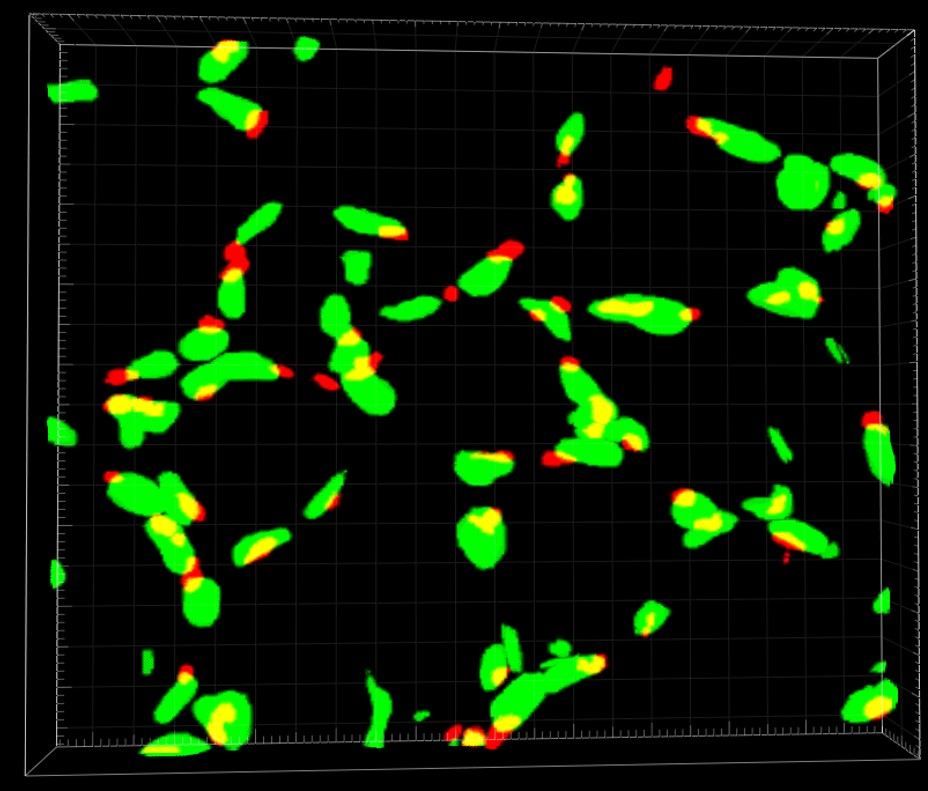
\includegraphics[width=5cm]{Images/2-mask-crop5.jpg}}\hfil
\subfigure[]{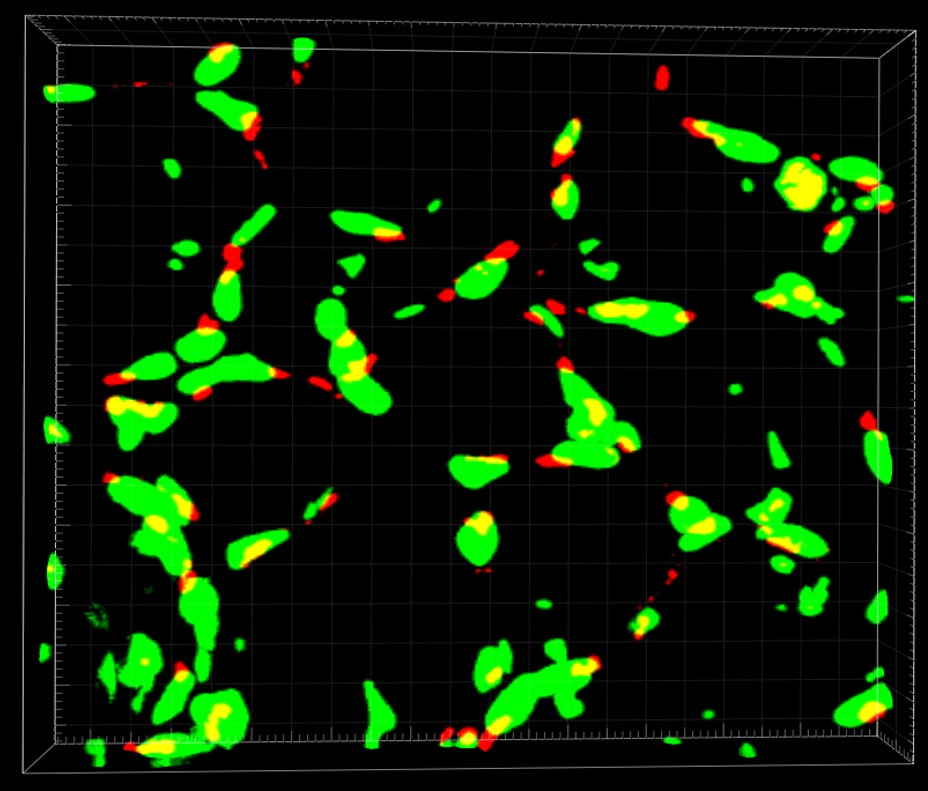
\includegraphics[width=5cm]{Images/vox2vox-2class-crop5.jpg}}

\subfigure[]{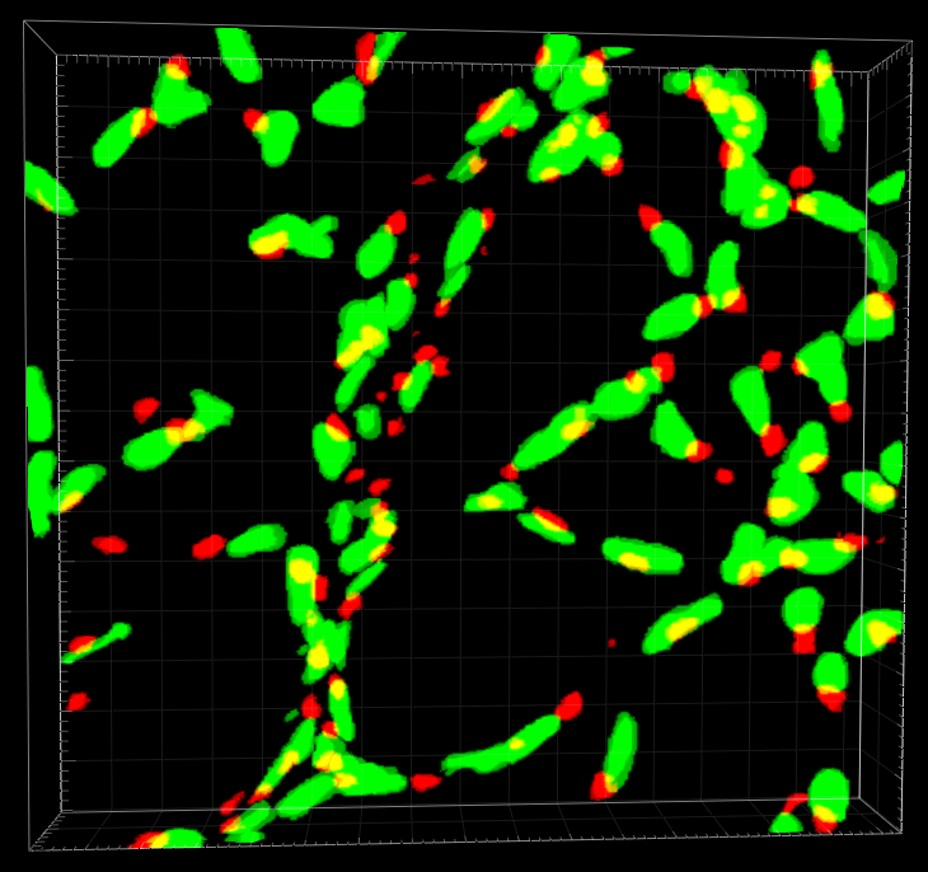
\includegraphics[width=5cm]{Images/2-mask-crop7.jpg}}\hfil 
\subfigure[]{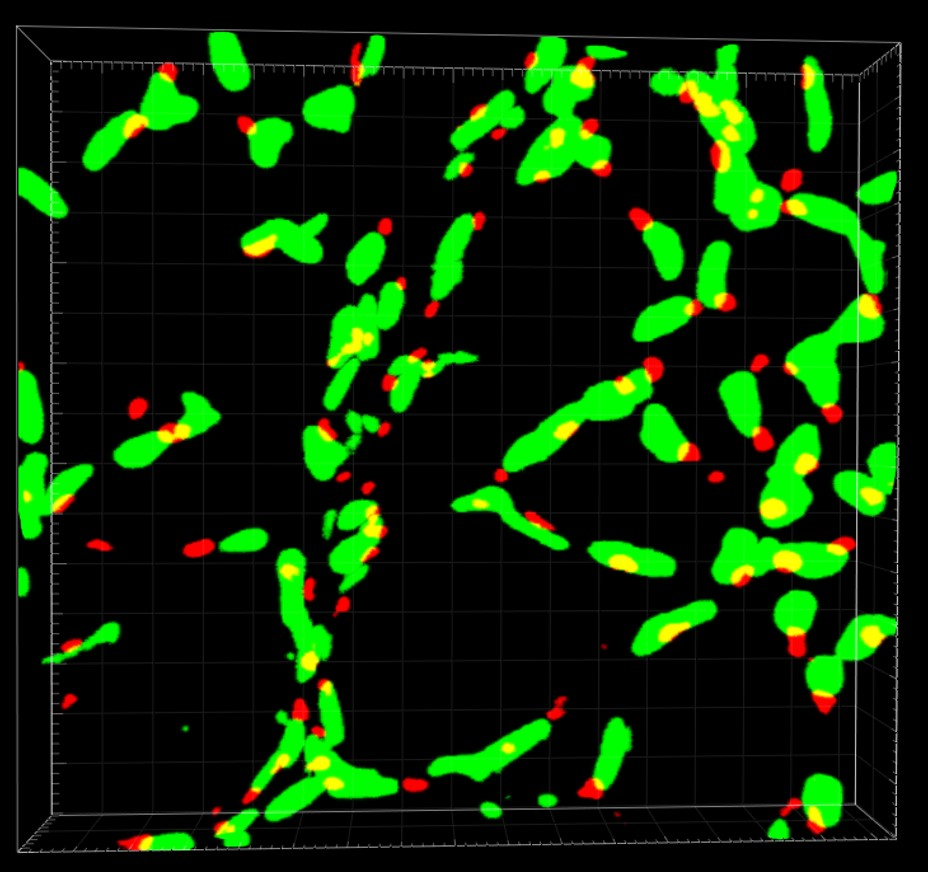
\includegraphics[width=5cm]{Images/vox2vox-2class-crop7.jpg}}

\caption{3D visualization of segmentation masks: (a) 3D ground truth $I^{gt}_{21}$; (b) 2 class Vox2Vox model tested on $I^{Pre}_1$; (c) 3D ground truth $I^{gt}_{22}$; (d) 2 class Vox2Vox model tested on $I^{Pre}_2$.}

\label{fig:results-vox2vox-2channel}

\end{figure}

From the results for the dice coefficient, we can conclude that the model is successful in identifying most of the nuclei and Golgi in the microscopic image volumes. For the Golgi segmentation mask, we verified in figure \ref{fig:results-vox2vox-2channel} that the model correctly identifies all Golgi. However, the margins for all Golgi are smaller than the ground truth segmentation mask, resulting in lower recall. This is likely due to the fact that the ground truth segmentation masks have low resolution, as shown in Figure \ref{fig:errors-unet} (c), and also to discontinuities in \ac{3D}, since these masks are created slide by slide in 2D. Consequently, the Vox2Vox model learns to generate images with this low resolution, which makes it difficult to segment the margins, especially of small objects like Golgi.

For the cell nuclei, we found that the model is very sensitive to noise in this class. This is particularly evident in the $I^{Pre}_1$ image test, as part of this image contains a lot of background noise for the nucleus channel and this noise is detected by the model, resulting in lower precision. However, this also results in the model being able to detect Golgi that are difficult to classify, i.e., Golgi with low contrast in the segmentation mask.


\subsubsection*{3 Class}

In this method, the number of output probability maps of Vox2Vox generator model is three, so we can classify the nuclei, Golgi and nucleus-Golgi pairs of the input images. All other parameters described in the implementation details are retained, except for the generator loss function, where we add another term to account for the Dice Loss of the nucleus-Golgi pairs class and set a gain $\beta_3$ = 1. The model was then trained using the pre-processed dataset and respective ground truth masks.

After training, the performance of the model is tested on the two microscopic image volumes $I^{Pre}_1$ and $I^{Pre}_2$. Figure \ref{fig:results-vox2vox-3channel} is a 3D visualization of the segmentation results for these volumes and table \ref{tab:results-3class-vox2vox} shows the average quantitative results.

\begin{table}[!htb]
\centering
\caption{Average metric values obtained from testing the 3 class Vox2Vox model on two pre-processed microscopic images}
\label{tab:results-3class-vox2vox}
\resizebox{\columnwidth}{!}{%
\renewcommand\arraystretch{1.4}
\begin{tabular}{|c|c|c|c|c|c|c|c|c|}
\hline
DC Nuclei & DC Golgi & DC Pair & Precision Nuclei & Precision Golgi & Precision Pair & Recall Nuclei & Recall Golgi & Recall Pair \\ \hline
0,7464    & 0,6720    & 0,7198 & 0,7170          & 0,6596          & 0,6763         & 0,7784        & 0,7204     & 0,7721      \\ \hline
\end{tabular}%
}
\end{table}

\begin{figure}[!htb]
\centering
\subfigure[]{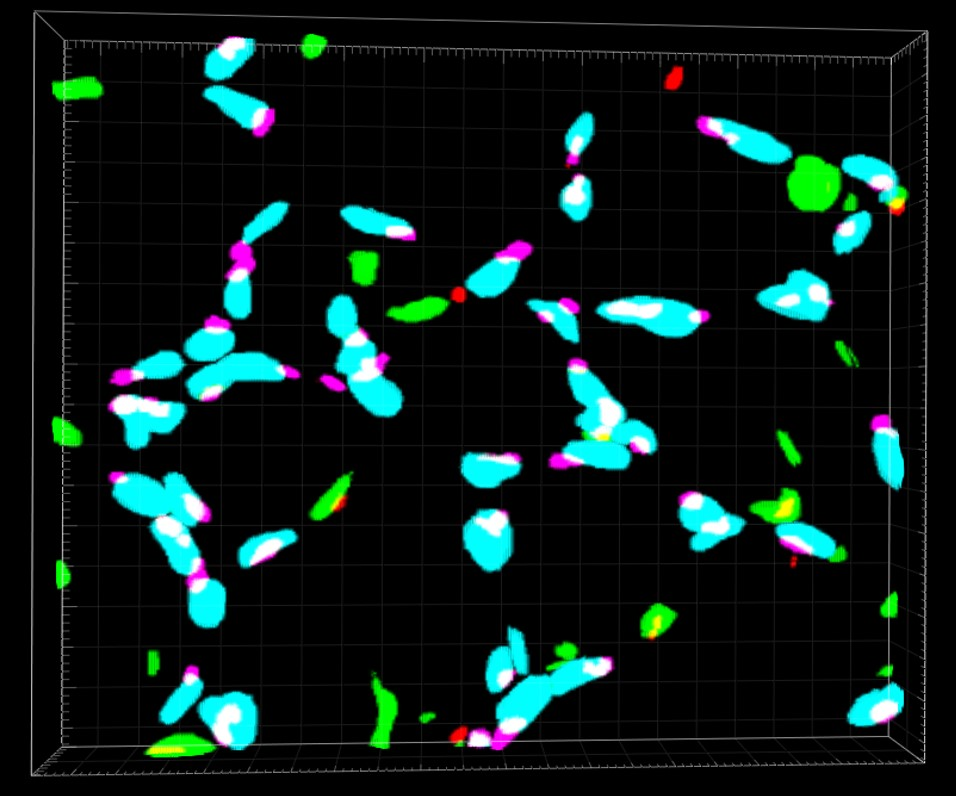
\includegraphics[width=5cm]{Images/3-mask-crop5-original.jpg}}\hfil
\subfigure[]{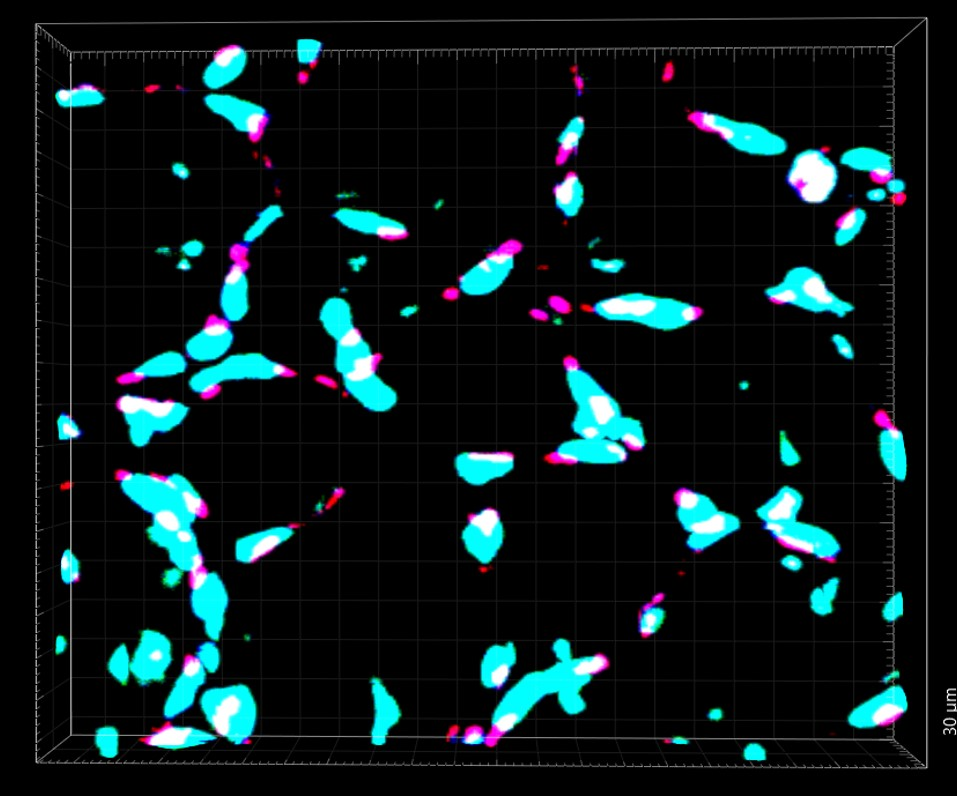
\includegraphics[width=5cm]{Images/vox2vox-3class-crop5.jpg}}

\subfigure[]{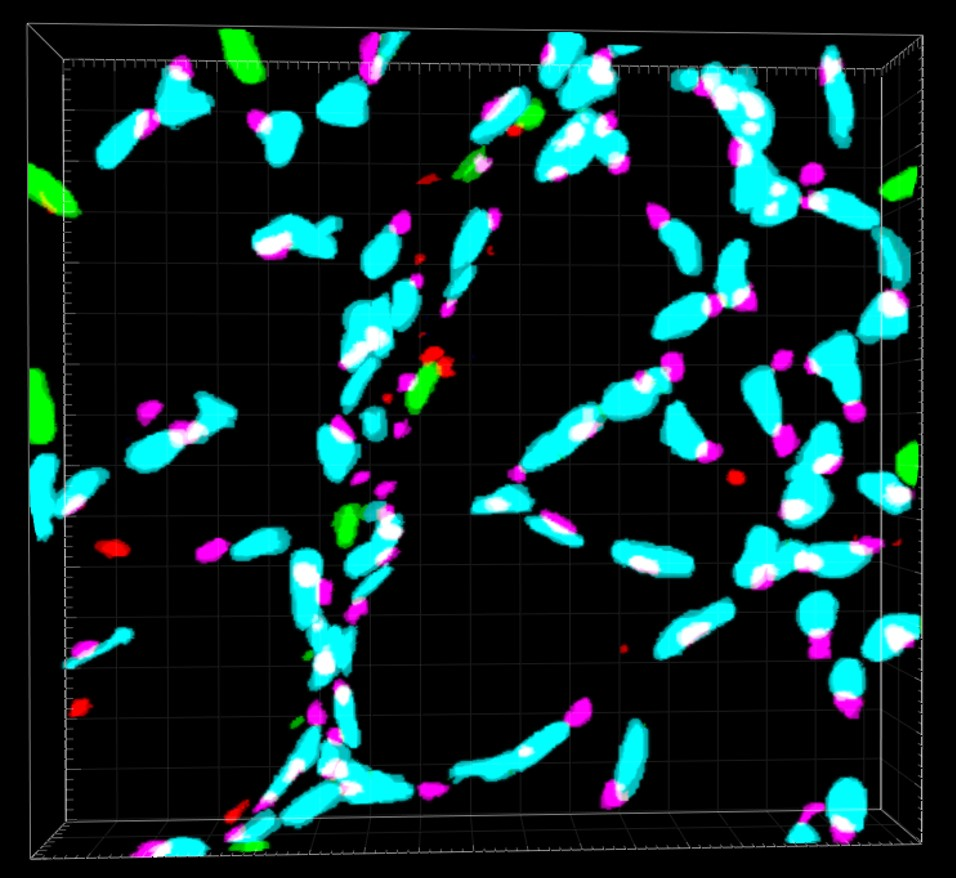
\includegraphics[width=5cm]{Images/3-mask-crop7-original.jpg}}\hfil 
\subfigure[]{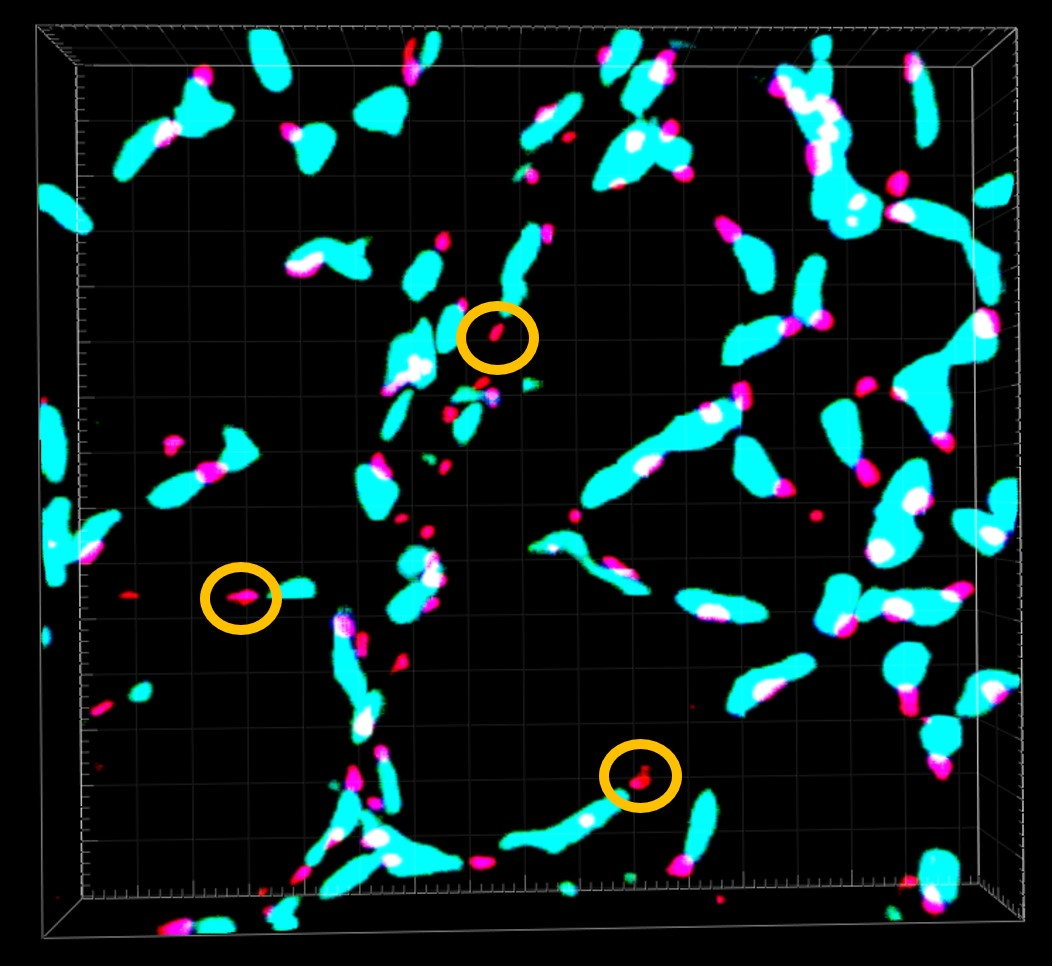
\includegraphics[width=5cm]{Images/vox2vox-3class-crop7.jpg}}

\caption{3D visualization of segmentation masks: (a) 3D ground truth $I^{gt}_{31}$; (b) 3 class Vox2Vox model tested on $I^{Pre}_1$; (c) 3D ground truth $I^{gt}_{32}$; (d) 3 class Vox2Vox model tested on $I^{Pre}_2$.}

\label{fig:results-vox2vox-3channel}

\end{figure}

If we compare the results presented in table \ref{tab:results-2class-vox2vox} and \ref{tab:results-3class-vox2vox} for the nuclei and Golgi classes, we verify that they remain relatively the same, as expected. Now, regarding the nucleus-Golgi pairs class, although the model is able to detect most of the nucleus-Golgi pairs in the images, the problem previously verified for the U-Net model remains in the Vox2Vox model, i.e., the model is not able to distinguish nucleus-Golgi pairs from individual nuclei and Golgi, which translates into lower precision. 

In figure \ref{fig:results-vox2vox-3channel} (d), it is highlighted by yellow circles that for this class, the model has difficulty segmenting small objects such as Golgi, which lowers the recall. This is also related to the fact that the ground truth segmentation masks have low resolution and the model learns to generate low resolution images as well.


\subsection{Proposed Approach - CycleGAN}

In this subsection the results obtained by training and testing the proposed unsupervised approach model CycleGAN are presented and discussed.

\subsubsection*{Implementation Details}

As mentioned in section \ref{section:proposed}, the CycleGAN model consists of four interconnected networks, two generators and two discriminators. After training, we keep only the generator corresponding to the segmentation network ($G_S$), the rest of the networks are used only to improve training. 

For training the CycleGAN we used: an initializer that generates weights with a normal distribution; the ADAM optimizer with a learning rate of 1e-3 and 5e-3 for the generators and discriminators, respectively; $\lambda_{cyc} = 10$ and $\lambda_{id} = 5$ in equation \ref{eq:total-cyclegan-loss} as proposed in \cite{cycleGAN:original} and a batch size of 2.

Specifically for the generators, the activation function \ac{Tanh} was used in the last layer so that the output has $n$-probability maps (where $n$ is the number of classes). Therefore, for these experiments, the input images had to be normalized to be in the range [-1,1]. Then the output images are normalized again to a range between [0,1]. For the segmentation network output ($G_S$), a threshold of 0.5 is then applied to each probability map to obtain the final segmentation mask volume.

During training, the performance of the model is tracked by using the generator models to generate translated versions of a few randomly selected images at the end of each epoch. The model is stopped when it reaches collapse mode, i.e., when it produces exactly the same output image for different input images. After training, we visually analyse the results obtained by CycleGAN for different epochs and select the model from the epoch that gives better results for the validation dataset.

Similar to Vox2Vox, we first trained the CycleGAN model by giving the Golgi and nuclei classes the same weight in the loss function. However, during training, we found that the model collapsed for the Golgi channel very quickly before it had a chance to improve. Therefore, similar to the Vox2Vox model, we changed the cycle consistency and identity loss to give more weight to the mean absolute error for Golgi. After some experiments the final weight given to this class was 3.5 and 1 to the nuclei class.


\subsubsection*{2 Class}

The CycleGAN was trained in two different ways: first in a supervised manner using the pre-processed microscopic image dataset together with the corresponding manually labelled segmentation masks to ensure the correct implementation of the model, and then in an unsupervised way with the synthetic segmentation mask dataset described in subsection \ref{subsection:synthetic_masks}. Then, both models were tested with the two microscopic image volumes $I^{Pre}_1$ and $I^{Pre}_2$. Figure \ref{fig:results-cyclegan-2channel} is a 3D visualization of the segmentation results for these volumes and table \ref{tab:results-2class-cyclegan} shows the average quantitative metrics.

% Please add the following required packages to your document preamble:
% \usepackage{graphicx}
\begin{table}[!htb]
\centering
\caption{Average metric values obtained from training the 2 class CycleGAN model in supervised and unsupervised way and testing these models on two pre-processed microscopic images}
\label{tab:results-2class-cyclegan}
\resizebox{\columnwidth}{!}{%
\renewcommand\arraystretch{1.4}
\begin{tabular}{c|c|c|c|c|c|c|}
\cline{2-7}
                                              & DC Nuclei & DC Golgi & Precision Nuclei & Precision Golgi & Recall Nuclei & Recall Golgi \\ \hline
\multicolumn{1}{|c|}{CycleGAN (Supervised)}   & 0,7612   & 0,6545  & 0,6894           & 0,6004        & 0,8528        & 0,7450     \\ \hline
\multicolumn{1}{|c|}{CycleGAN (Unsupervised)} & 0,7664    & 0,6427   & 0,6903           & 0,5468          & 0,8629        & 0,8038       \\ \hline
\end{tabular}%
}
\end{table}

\begin{figure}[!htb]
\centering
\subfigure[]{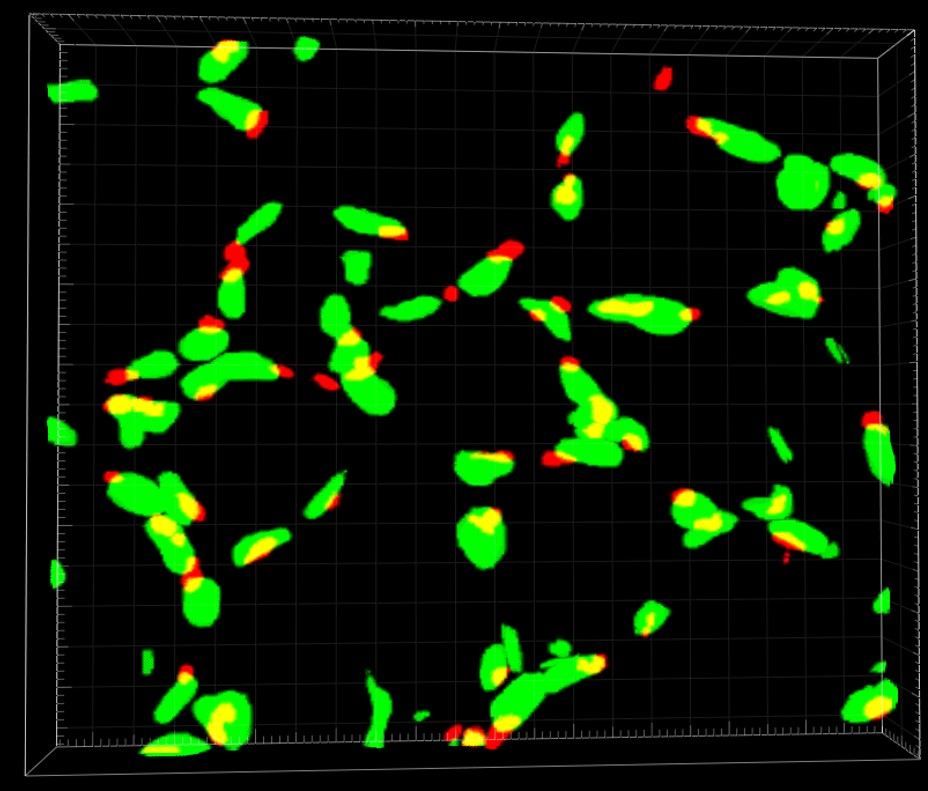
\includegraphics[width=5cm]{Images/2-mask-crop5.jpg}}\hfil
\subfigure[]{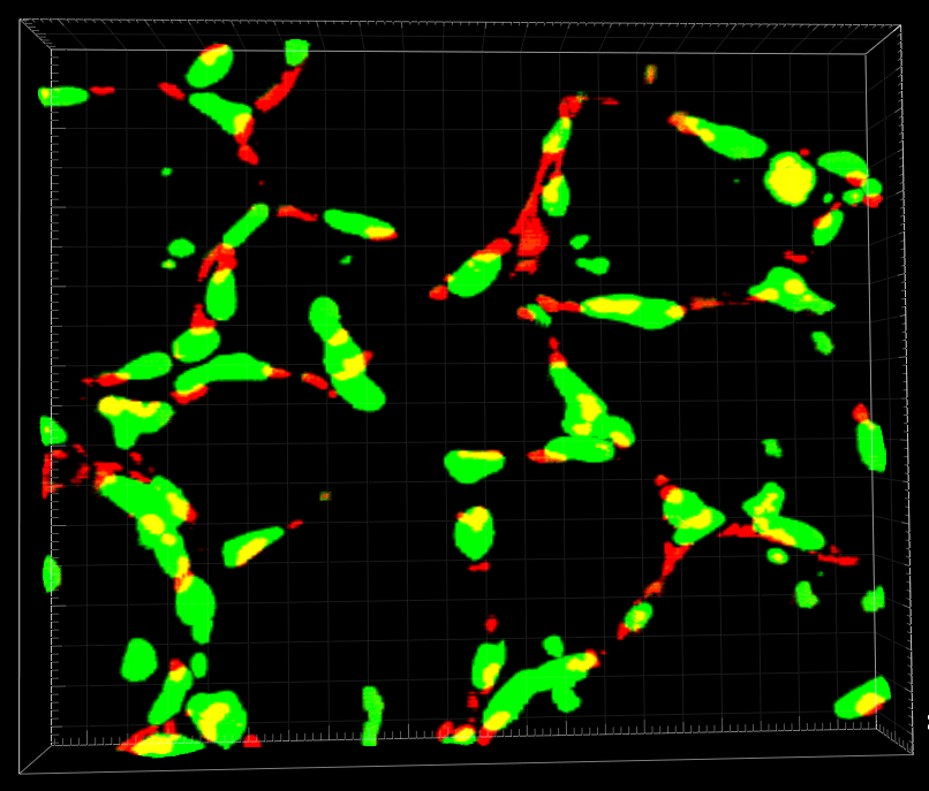
\includegraphics[width=5cm]{Images/cyclegan-2class-crop5-real.jpg}}\hfil 
\subfigure[]{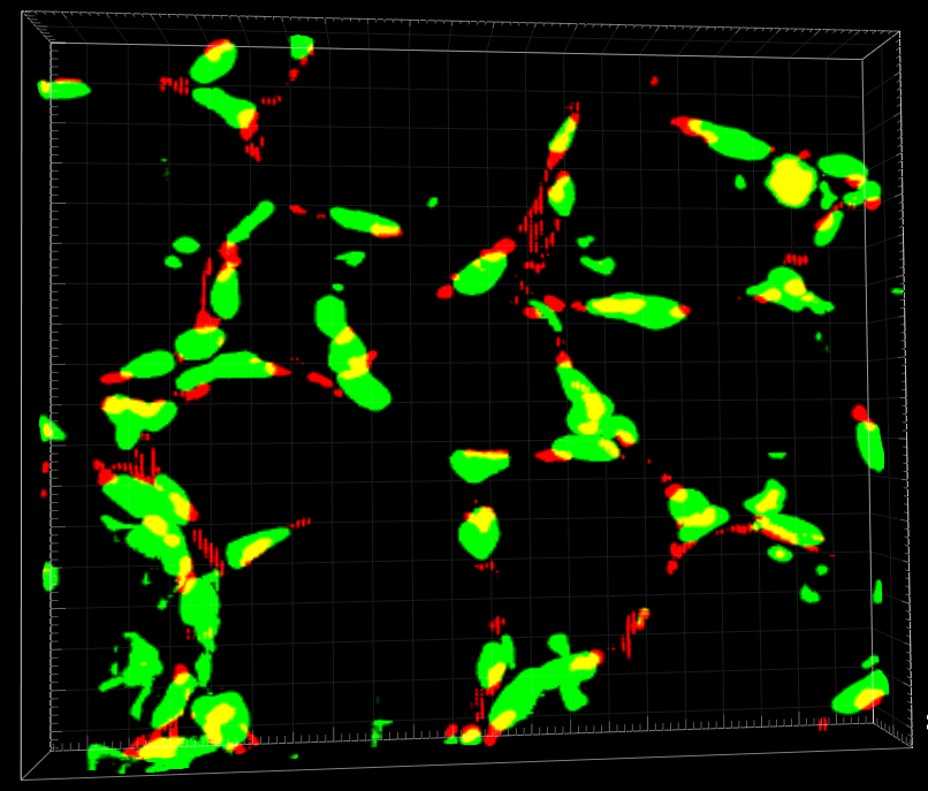
\includegraphics[width=5cm]{Images/cyclegan-2class-crop5.jpg}} 

\subfigure[]{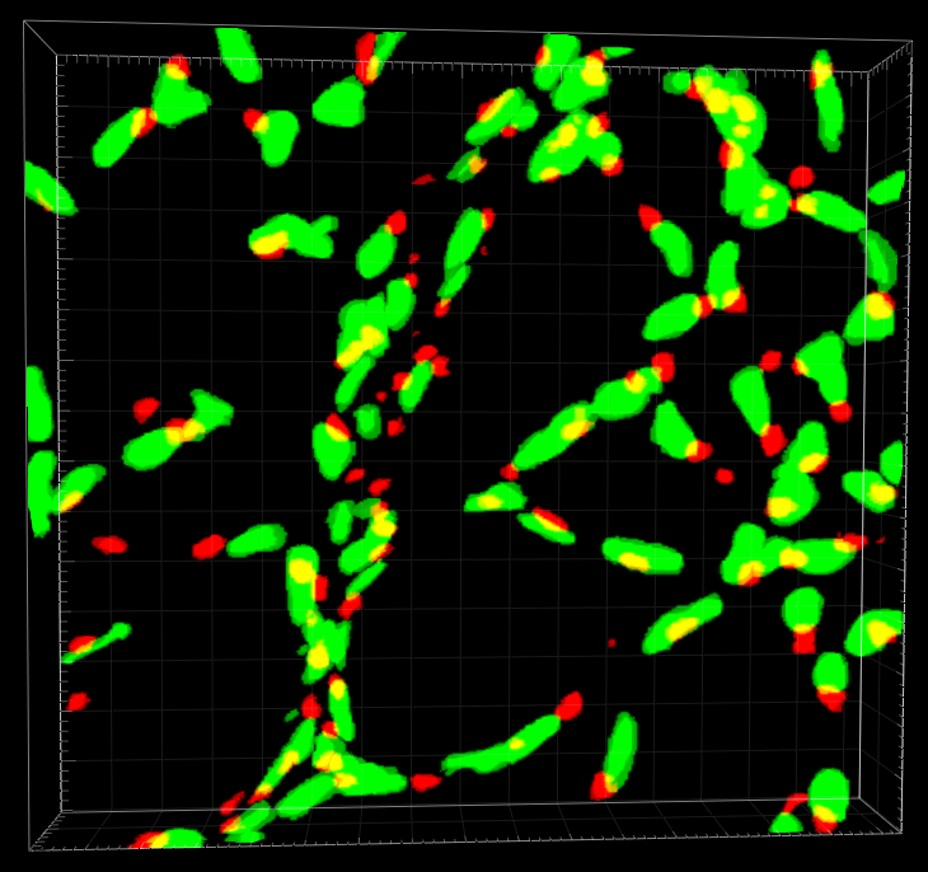
\includegraphics[width=5cm]{Images/2-mask-crop7.jpg}}\hfil
\subfigure[]{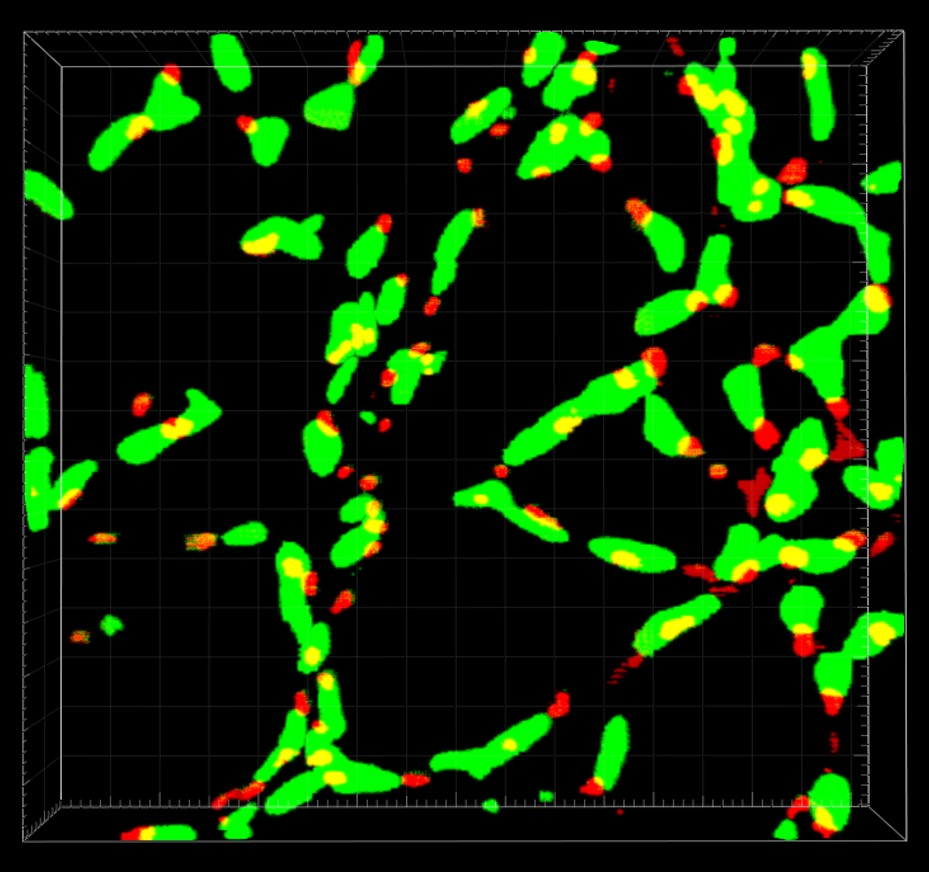
\includegraphics[width=5cm]{Images/cyclegan-2class-crop7-real.jpg}}\hfil
\subfigure[]{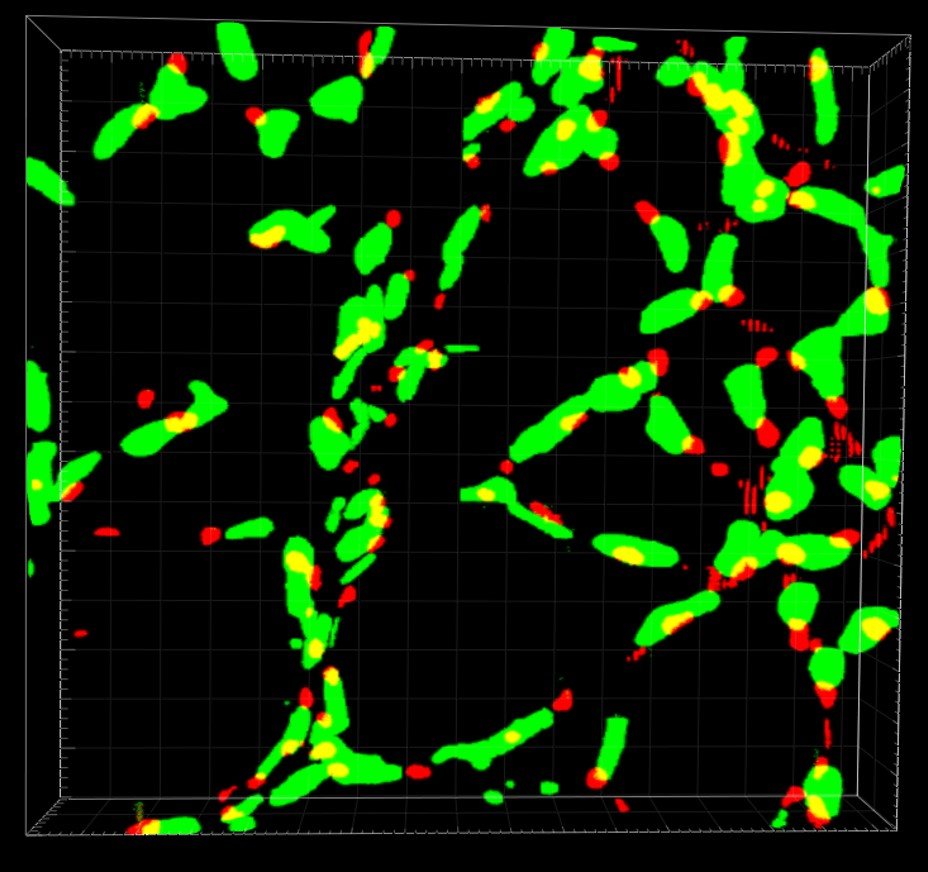
\includegraphics[width=5cm]{Images/cyclegan-2class-crop7.jpg}} 

\caption{3D visualization of segmentation masks: (a) 3D ground truth $I^{gt}_{21}$; (b) 2 class supervised CycleGAN model tested on $I^{Pre}_1$; (c) 2 class unsupervised CycleGAN model tested on $I^{Pre}_1$; (d) 3D ground truth $I^{gt}_{22}$; (e) 2 class supervised CycleGAN model tested on $I^{Pre}_2$; (f) 2 class unsupervised CycleGAN model tested on $I^{Pre}_2$.}

\label{fig:results-cyclegan-2channel}

\end{figure}

Based on figures \ref{fig:results-cyclegan-2channel} (b) and (e), we can verify that the supervised CycleGAN model successfully detects almost all nuclei and Golgi in the images. The advantage of this model is that, even if trained in a supervised manner, it does not require pairing of the microscopic image and the corresponding segmentation mask during training. 

From figures \ref{fig:results-cyclegan-2channel} (b) and (e), we can also observe that the supervised CycleGAN model for the class of nuclei has difficulty detecting some nuclei that have low contrast in the microscopic images, which affects recall, and that it is very sensitive to digital noise, which affects the value of the precision. The same problems occur with the Golgi class, but are intensified due to the small size of the Golgi, which makes it difficult for the model to learn to detect it correctly and especially to segment well the borders.

If we now analyse the results of the unsupervised CycleGAN model, we find that, like the supervised model, it correctly detects almost all nuclei and Golgi in the images. From table \ref{tab:results-2class-cyclegan}, we verified that the results for the supervised and unsupervised CycleGAN models are very close. This suggests that the problems exhibited by the CycleGAN model are due only to the limitations of the model and not to the use of synthetic masks instead of the real ones to train the model. Actually, it has been verified that the model does not learn to generate masks with low resolution, as is the case with the supervised model, because the synthetic masks have better resolution than the manually labelled masks.


\subsubsection*{3 Channel}

In this method, the number of output probability maps for the CycleGAN generator networks is three, so we can classify the nuclei, Golgi, and nucleus-Golgi pairs of the input images. All other parameters described in the implementation details are kept, except for cycle consistency and identity, where we add another term to account for the mean absolute error of the nucleus-Golgi pair class, and set a gain equal to 1. The model was then trained with the pre-processed dataset and synthetic segmentation masks described in subsection \ref{subsection:synthetic_masks}.

After training, the performance of the model is tested on the two microscopic image volumes $I^{Pre}_1$ and $I^{Pre}_2$. Figure \ref{fig:results-cycleGAN-3channel} is a 3D visualization of the segmentation results for these volumes and table \ref{tab:results-3class-cycleGAN} shows the average quantitative results.

% Please add the following required packages to your document preamble:
% \usepackage{graphicx}
\begin{table}[!htb]
\centering
\caption{Average metric values obtained from testing the 3 class unsupervised CycleGAN model on two pre-processed microscopic images}
\label{tab:results-3class-cycleGAN}
\resizebox{\columnwidth}{!}{%
\renewcommand\arraystretch{1.4}
\begin{tabular}{|c|c|c|c|c|c|c|c|c|}
\hline
DC Nuclei & DC Golgi & DC Pair & Precision Nuclei & Precision Golgi & Precision Pair & Recall Nuclei & Recall Golgi & Recall Pair \\ \hline
0,7261    & 0,5942   & 0,6999  & 0,7174           & 0,5874          & 0,6711         & 0,7366        & 0,6133       & 0,7314      \\ \hline
\end{tabular}%
}
\end{table}

\begin{figure}[!htb]
\centering
\subfigure[]{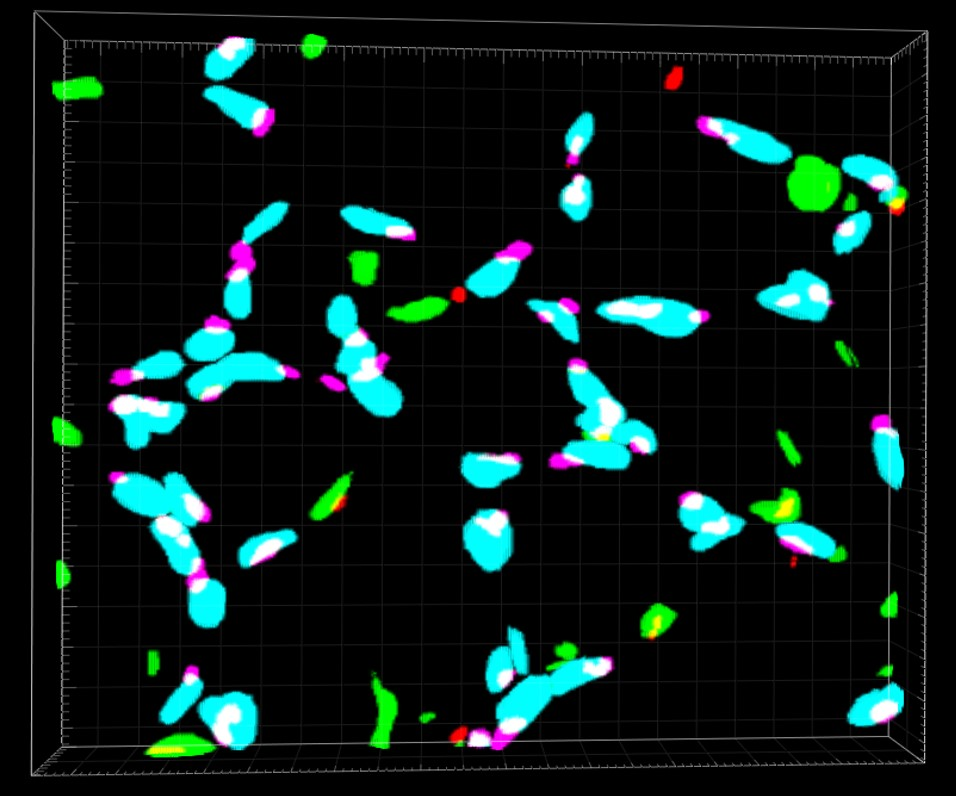
\includegraphics[width=5cm]{Images/3-mask-crop5-original.jpg}}\hfil
\subfigure[]{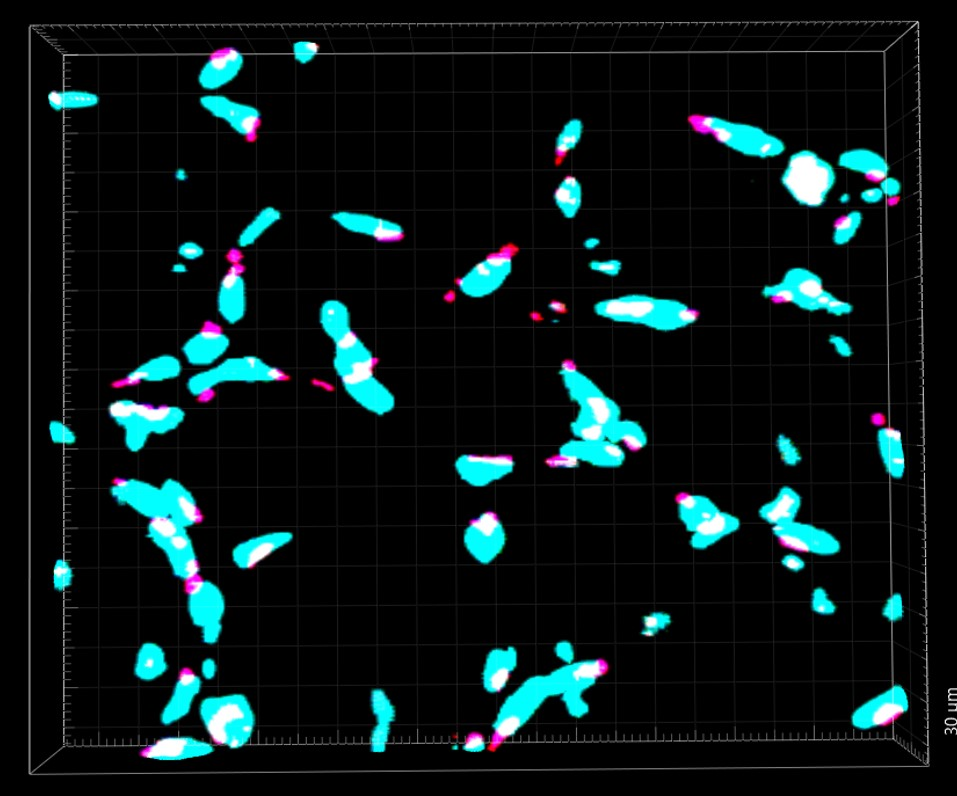
\includegraphics[width=5cm]{Images/cyclegan-3class-crop5.jpg}}

\subfigure[]{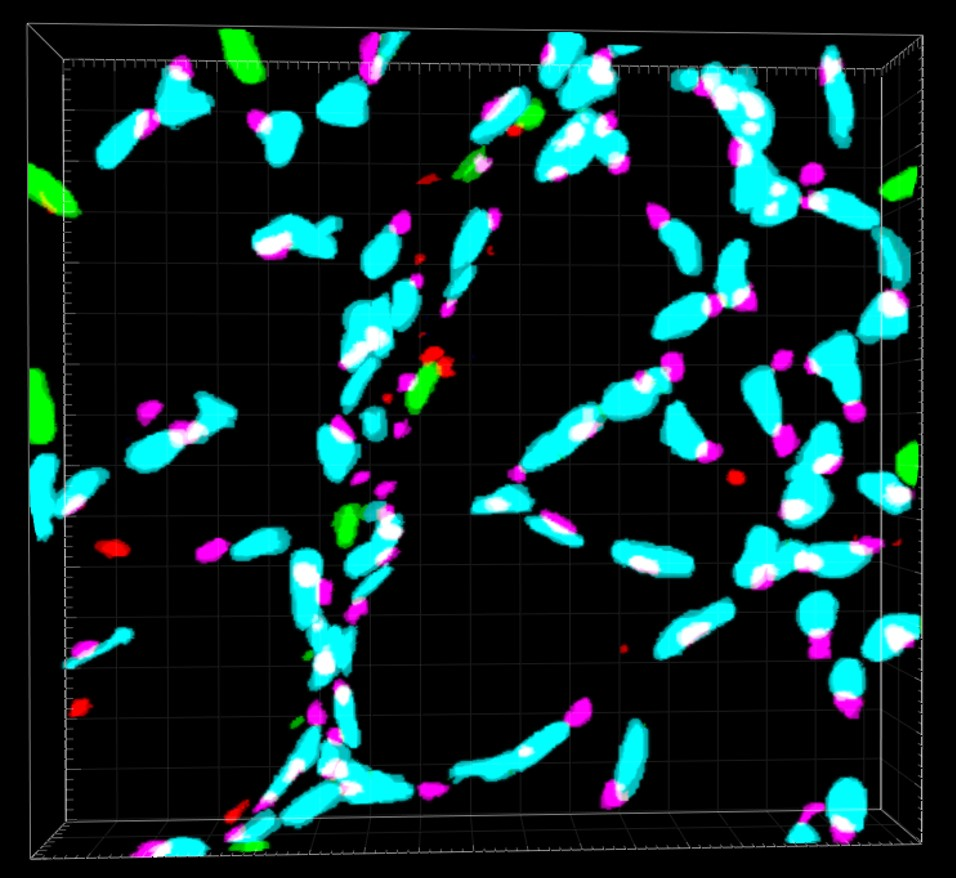
\includegraphics[width=5cm]{Images/3-mask-crop7-original.jpg}}\hfil 
\subfigure[]{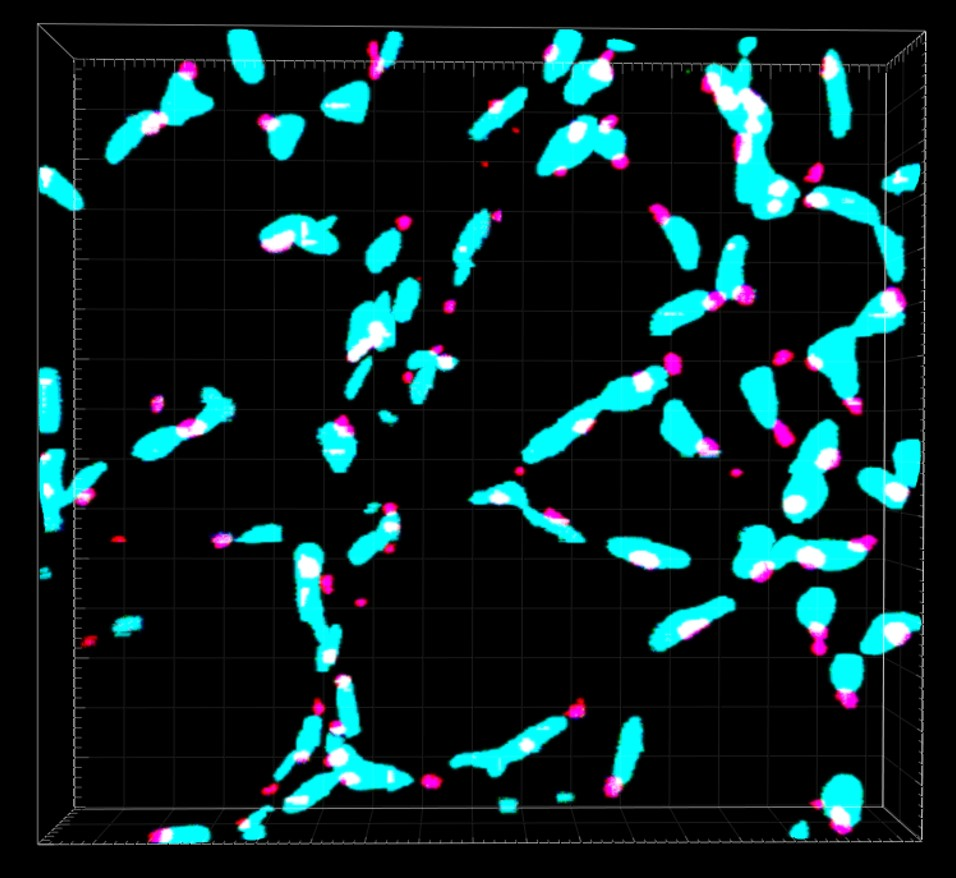
\includegraphics[width=5cm]{Images/cyclegan-3class-crop7.jpg}}

\caption{3D visualization of segmentation masks: (a) 3D ground truth $I^{gt}_{31}$; (b) 3 class unsupervised CycleGAN model tested on $I^{Pre}_1$; (c) 3D ground truth $I^{gt}_{32}$; (d) 3 class unsupervised CycleGAN model tested on $I^{Pre}_2$.}

\label{fig:results-cycleGAN-3channel}



\end{figure}

From figure \ref{fig:results-cyclegan-2channel} and \ref{fig:results-cycleGAN-3channel}, we can observe that the model is less sensitive to digital noise and background clutter which is reflected in an improvement in precision for the nuclei and Golgi classes. However, it has more difficulty in detecting all nuclei and Golgi in the images 

For the nuclei-Golgi pairs class, we can also see in figure \ref{fig:results-cycleGAN-3channel} that, as with the previous U-Net and Vox2Vox models, the model is unable to distinguish isolated nuclei and Golgi from paired ones, but it can detect most pairs in the image. An effect that was also confirmed is that for some isolated nuclei, the model generates a Golgi inside the nucleus instead of simply not classifying it as a pair.

\subsection{Execution time}
\label{subsection:execution-time}

In this section, we present the time needed to train and test the models. As mentioned earlier, we have a total of 8 crops for training and testing the models. Where 6 of these crops are used to train the models and 2 of them are used for testing. It was estimated how long it takes to manually label nuclei and Golgi in a crop. The estimate was 28 hours. For training and testing time, the time needed to obtain these crops was considered. In the case of CycleGAN, the training time was added to the time needed to create the synthetic masks (40 minutes). The final values are presented in table \ref{tab:time}.

\begin{table}[!htb]
\centering
\caption{Time needed to train and test the models}
\label{tab:time}
\renewcommand\arraystretch{1.4}
\begin{tabular}{c|c|c|c|}
\cline{2-4}
                                    & U-Net                  & Vox2Vox                & CycleGAN               \\ \hline
\multicolumn{1}{|c|}{Training Time} & (28h * 6) + 66 min     & (28h * 6) + 74 min     & 40 min + 28,6 h        \\ \hline
\multicolumn{1}{|c|}{Testing Time}  & (28h * 2) + 35 seconds & (28h * 2) + 35 seconds & (28h * 2) + 35 seconds \\ \hline
\multicolumn{1}{|c|}{Total Time}    & 225,1 hours            & 225,23 hours           & 85,3 hours             \\ \hline
\end{tabular}
\end{table}



\subsection{Comparison between approaches}

In this section, the segmentation results obtained with the supervised models U-Net and Vox2Vox are compared with the proposed unsupervised model CycleGAN. The results obtained for each class nuclei, Golgi and nucleus-Golgi pair are analysed separately.

\begin{table}[!htb]
  \centering
  \caption{Average results obtained for the three different models tested}
  \label{tab:results-all}
  \renewcommand\arraystretch{1.4}
  \resizebox{\columnwidth}{!}{%
  \begin{tabular}{l|c|c|c|c|c|c|}
  \cline{2-7}
                                 & DC Nuclei & DC Golgi & Precision Nuclei & Precision Golgi & Recall Nuclei & Recall Golgi \\ \hline
  \multicolumn{1}{|l|}{U-Net}    & 0,7775    & 0,6938   & 0,7067           & 0,6500          & 0,8692        & 0,7683       \\ \hline
  \multicolumn{1}{|l|}{Vox2Vox}  & 0,7539    & 0,6883   & 0,6529           & 0,7078          & 0,8933        & 0,6917       \\ \hline
  \multicolumn{1}{|l|}{CycleGAN} & 0,7664    & 0,6427   & 0,6903           & 0,5468          & 0,8629        & 0,8038       \\ \hline
  \end{tabular}%
  }
\end{table}

Segmentation of the nuclei class is challenging because the microscopic images have some background clutter and some of the nuclei have low contrast in the images. For this class, the best dice coefficient was obtained for the U-Net model with 0,7775, but CycleGAN obtained a similar result with 0,7612 and then Vox2Vox with 0,7464. The precision and recall values for the CycleGAN and U-Net models are also very close, with the CycleGAN model only being inferior by less than one percent. The lower dice coefficient of Vox2Vox is due to its high sensitivity to digital noise, which explains its relatively low precision of 0,6529. However, it is the best of the 3 models at detecting Golgi, as it can detect and segment nuclei even when they have low contrast.

The challenges in classifying the Golgi class are mainly: the digital noise coming from particles such as dust entering the analysed sample and producing blurs (due to their autofluorescence) with high contrast in the red channel of the microscopic images, which can be mistaken for Golgi; and the small size of the Golgi, which makes detection and boundary segmentation difficult. For this class, the best dice coefficient was obtained for the U-Net model with 0,6938, followed by the Vox2Vox model with 0,6883 and the CycleGAN model with 0,6427. Although the U-Net model had the best Dice Coefficient, because it was able to detect and segment the Golgi best on average, the Vox2Vox model obtained the best precision with 0,7078 and CycleGAN the best recall with 0,8038. Analysing the segmentation masks obtained for these models, we can conclude that the Vox2Vox model best segments the boundaries of the nuclei it detects and CycleGAN is the model that detects the most Golgi on the images.



For the nucleus-Golgi pair class, the main classification challenge is that some nuclei and Golgi do not form a pair and not all nucleus and Golgi of a pair overlap. For this class, the best dice coefficient was obtained for the U-Net with 0,7601, followed by the Vox2Vox model with 0,7198 and then CycleGAN with 0,6999. In terms of accuracy, all the models are very close to each other as they all have the same problem of incorrectly detecting individual nuclei and Golgi as being paired. However, the best model at detecting the pairs on the image is the U-Net. Probably the Vox2Vox model and CycleGAN should be more complex (more kernels or more layers) to be able to better segment this class.

As mentioned earlier, supervised models are highly dependent on the data on which they are trained. If these data have errors or are imperfect, these imperfections are propagated to the models. We have found that the ground-truth masks have problems, such as not all objects are segmented and the masks have low resolution. Also, it is very difficult to obtain these masks. With the CycleGAN model, we were able to obtain comparable results to the supervised models in less than half the time, as demonstrated in section \ref{subsection:execution-time}. Since this model does not require extensive manual work and also has the advantage of being more transferable, i.e., it does not depend so much on the data on which it is trained, it learns better the actual distribution of the data.